%% ========================================================================
%%%% Basic settings
%% ========================================================================
%% (idea of using newcommands for basic documentclass settings from: Thomas Schlager)

\newcommand{\mypapersize}{A4}
%% e.g., "A4", "letter", "legal", "executive", ...
%% The size of the paper of the resulting PDF file.

\newcommand{\mylaterality}{oneside}
%% "oneside" or "twoside"
%% Either you are creating a document which is printed on both, left pages
%% and right pages (twoside) or you create a document which is printed
%% on right pages only (oneside).

\newcommand{\mydraft}{false}
%% "true" or "false"
%% Use draft mode? If true, included graphics are replaced by empty
%% rectangles (of same size) and overfull boxes (in margin space) are
%% marked with black box (-> easy to spot!)

\newcommand{\myparskip}{half}
%% e.g., "no", "full", "half", ...
%% How to separate paragraphs: indention ("no") or spacing ("half",
%% "full", ...).

\newcommand{\myBCOR}{0mm}
%% Inner binding correction. This value depends on the method which is
%% being used to bind your printed result. Some techniques do not
%% require a binding correction at all ("0mm"), other require for
%% example "5mm". Refer to KOMA script documentation for a detailed
%% explanation what a binding correction is and how to measure it.

\newcommand{\myfontsize}{12pt}
%% e.g., 10pt, 11pt, 12pt
%% The font size of the main text in pt (points).

\newcommand{\mylinespread}{1.0}
%% e.g., 1.0, 1.5, 2.0
%% Line spacing in %/100. For example 1.5 means 150% of the usual line
%% spacing. Please use with caution: 100% ("1.0") is fine because the
%% font was designed for it.

\newcommand{\mylanguage}{american,ngerman}
%% "english,ngerman", "ngerman,english", ...
%% NOTE: The *last* language is the active one!
%% See babel documentation for further details.

%% BibLaTeX-settings: (see biblatex reference for further description)
\newcommand{\mybiblatexstyle}{numeric}
%% e.g., "alphabetic", "authoryear", ...
%% The biblatex style which is being used for referencing. See
%% biblatex documentation for further details and more values.
%%
%% CAUTION: if you change the style, please check for (in)compatible
%%          "biblatex" package options in the file
%%          "template/preamble.tex"! For example: "alphabetic" does
%%          not have an option "dashed=..." and causes an error if it
%%          does not get removed from the list of options.

\newcommand{\mybiblatexdashed}{false}  %% "true" or "false"
%% If true: replace recurring reference authors with a dash.

\newcommand{\mybiblatexbackref}{true}  %% "true" or "false"
%% If true: create backward links from reference to citations.

\newcommand{\mybiblatexfile}{references-biblatex.bib}
%% Name of the biblatex file that holds the references.

%\newcommand{\mydispositioncolor}{30,103,182}
\newcommand{\mydispositioncolor}{0,0,0}
%% e.g., "30,103,182" (blue/turquois), "0,0,0" (black), ...
%% Color of the headings and so forth in RGB (red,green,blue) values.
%% NOTE: if you are using "0,0,0" for black, printers might still
%%       recognize pages as color pages. In case this is a problem
%%       (paying for color print-outs vs. paying for b/w-printouts)
%%       please edit file "template/preamble.tex" and change
%%       "\definecolor{DispositionColor}{RGB}{\mydispositioncolor}"
%%       to "\definecolor{DispositionColor}{gray}{0}" and thus
%%       overwriting the value of \mydispositioncolor above.

\newcommand{\mycolorlinks}{true}  %% "true" or "false"
%% Enables or disables colored links (hyperref package).

\newcommand{\mytitlepage}{template/title_VWA}
%% Your own or one of following pre-defined title pages:
%% "template/title_plain_maketitle": simple maketitle page
%% "template/title_Diplomarbeit_KF_Uni_Graz.tex": fancy (german) title page for KF Uni Graz
%% "template/title_Thesis_TU_Graz":
%%             titlepage for Graz University of Technology (correct
%%             (old?) Corporate Design) by Karl Voit (2012)
%% "template/title_Thesis_TU_Graz_-_kazemakase":
%%             titlepage for Graz University of Technology
%%             (correct new Corporate Design) by kazemakase (2013):
%%             see https://github.com/novoid/LaTeX-KOMA-template/issues/5
%% "template/title_VWA": titlepage for Vorwissenschaftliche Arbeit

\newcommand{\mytodonotesoptions}{}
%% e.g., "" (empty), "disable", ...
%% Options for the todonotes-package. If "disable", all todonotes will
%% be hidden (including listoftodos).

%% Load main settings for document preamble:

  
\input{template/preamble}%% DO NOT REMOVE THIS LINE!

\setboolean{myaddcolophon}{true}  %% "true" or "false"
%% If set to "true": a colophon (with notes about this document
%% template, LaTeX, ...) is added after the title page.
%% Please do not set to "false" without a good reason. The colophon
%% helps your readers to get in touch with LaTeX and to find this template.

\setboolean{myaddlistoftodos}{false}  %% "true" or "false"
%% If set to "true": the current list of open todos is added after the
%% table of contents. If \mytodonotesoptions is set to "disable", no
%% list of todos is added, independent of this setting here.

\setboolean{english_affidavit}{true}  %% "true" or "false"
%% If set to "true": the language of the statutory declaration text is set to
%% English, otherwise it is in German.


%% ========================================================================
%%%% Document metadata
%% ========================================================================

%% general metadata:
\newcommand{\myauthor}{Florian Kluibenschedl}  %% also used for PDF metadata (hyperref)
\newcommand{\myauthorwithexistingtitles}{\myauthor{}, OLDDEGREE}  %% including
                                %% university degree already held
                                %% (BSc, MSc, ...)
\newcommand{\mytitle}{Direkte Analyse von Chlorophyllkataboliten}  %% also used for PDF metadata (hyperref)
\newcommand{\mysubject}{Chemie}  %% also used for PDF metadata (hyperref)
\newcommand{\mykeywords}{Chemie}  %% also used for PDF metadata (hyperref)

%% this information is used only for generating the title page:
\newcommand{\myworktitle}{Master's Thesis}  %% official type of work like ``Master theses''
\newcommand{\mygrade}{Master of Science} %% title you are getting with this work like ``Master of ...''
\newcommand{\mystudy}{8a} %% your study like ``Arts''
\newcommand{\mydegreeprogramme}{Master's degree programme: \mystudy} %% Master's or PhD degree programme
\newcommand{\myuniversity}{Graz University of Technology} %% your university/school
\newcommand{\myinstitute}{BRG Telfs} %% affiliation
\newcommand{\myinstitutehead}{Univ.-Prof.\,Dipl-Ing.\,Dr.techn.~Some One} %% head of institute
\newcommand{\mysupervisor}{Mag. Mathias Scherl} %% your supervisor
\newcommand{\myevaluator}{Prof.~Some Genius} %% your evaluator
\newcommand{\myhomestreet}{Weißenbachgasse 37} %% your home street (with house number)
\newcommand{\myhometown}{Telfs} %% your home town
\newcommand{\myhomepostalnumber}{6410} %% your postal number of home town
\newcommand{\mysubmissionmonth}{Februar} %% month you are handing in
\newcommand{\mysubmissionyear}{2018} %% year you are handing in
\newcommand{\mysubmissiontown}{\myhometown} %% town of handing in (or \myhometown)

%% additional information for generic_documentation title page
\newcommand{\myid}{1234567} %% Matrikelnummer
\newcommand{\mylecture}{LECTURE} %%


%% ========================================================================
%%%% MISC command definitions
%% ========================================================================
\input{template/mycommands}

%% ========================================================================
%%%% Typographic settings
%% ========================================================================
\input{template/typographic_settings}


%% ========================================================================
%%%% MISC usepackages
%% ========================================================================

%% ... it's OK to put here your own usepackage commands ...
\usepackage{chemfig,chemmacros}
\usepackage{graphicx}
\usepackage{amsmath,amssymb,amsthm,textcomp}
\usepackage{enumerate}
\usepackage{multicol}
\usepackage{tikz}
\usepackage{geometry}
\usepackage{tabu}
\usepackage{siunitx}
%\usepackage{subfig}
\usepackage{caption}
\usepackage{subcaption}
\usepackage{tabu}

\usepackage{listings}

\usepackage{rotating}
\usepackage{tabularx}

\usepackage{booktabs}
\usepackage{colortbl}
\usepackage{xcolor}
\usepackage{xfrac}
\usepackage[export]{adjustbox}[2011/08/13]

\newcommand{\ra}[1]{\renewcommand{\arraystretch}{#1}}

%% ========================================================================
%%%% MISC self-defined commands and settings
%% ========================================================================

%% ... it's OK to put here your own newcommand/newenvironment-definitions ...
\newcounter{oldtocdepth}

\newcommand{\hidefromtoc}{%
  \setcounter{oldtocdepth}{\value{tocdepth}}%
  \addtocontents{toc}{\protect\setcounter{tocdepth}{-10}}%
}

\newcommand{\unhidefromtoc}{%
  \addtocontents{toc}{\protect\setcounter{tocdepth}{\value{oldtocdepth}}}%
}


\newcommand{\myLaT}{\LaTeX{}@TUG\xspace} %% LaTeX@TUG text "logo"

\hyphenation{ex-am-ple hy-phen-ate}  %% in order to use German umlauts
%% here (Ver-\"of-fent-li-chung), you have to check for
%% activated \usepackage[T1]{fontenc} in the preamble

%% override default language of babel: (be sure to know, what you're
%% doing here)
%\selectlanguage{american}
%\selectlanguage{ngerman}

%% ========================================================================
%%%% Templates
%% ========================================================================

%% template for inserting figures:
% \myfig{}%% filename
%       {}%% width/height
%       {}%% caption
%       {}%% optional (short) caption for list of figures
%       {fig:}%% label

%% acronyms in small caps: \myacro{UNESCO}


\input{template/pdf_settings}  %% should be *last* definitions in preamble!
%% ========================================================================
%%%% begin{document}
%% ========================================================================
\begin{document}

%\frontmatter                    %% KOMA: roman page numbers and such; only available in scrbook

%\begin{titlepage}[htbp!]
%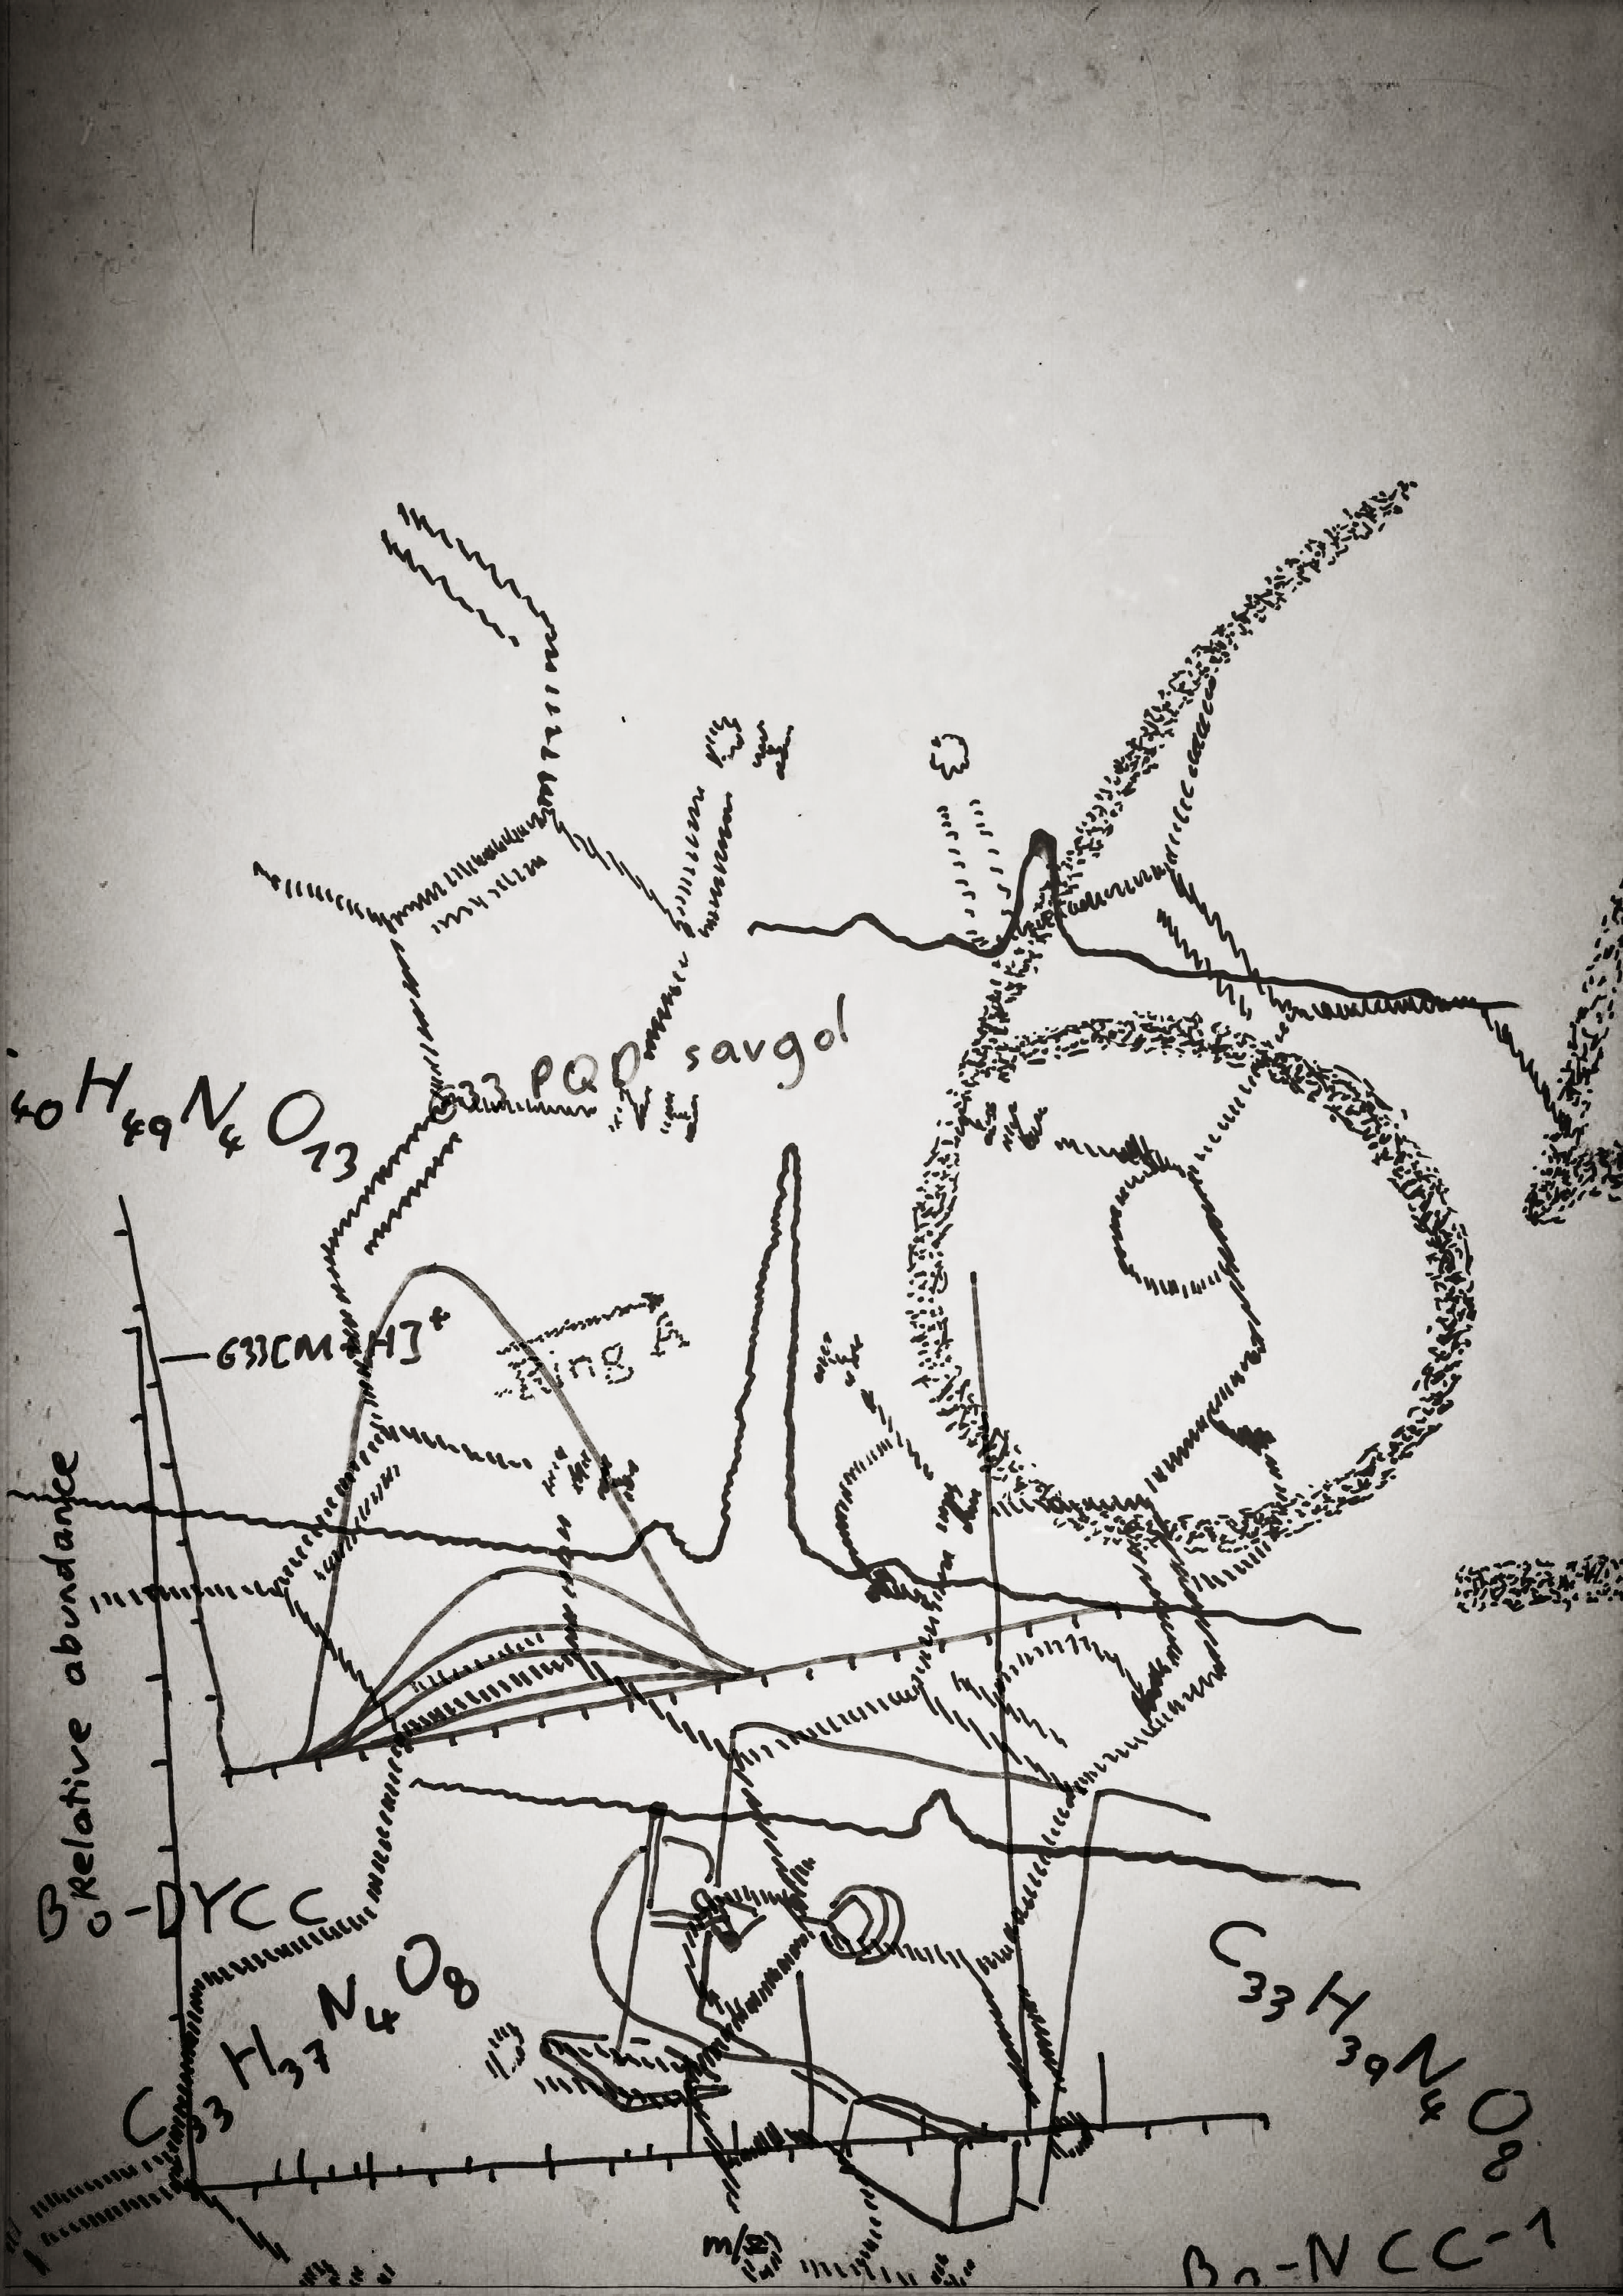
\includegraphics[width=\paperwidth, height=\paperheight]{template/VWA_Titelblatt_selected.png}
%\end{titlepage}

\thispagestyle{empty}
  \begin{tikzpicture}[remember picture, overlay]
    \node[inner sep=0pt] at (current page.center) {
      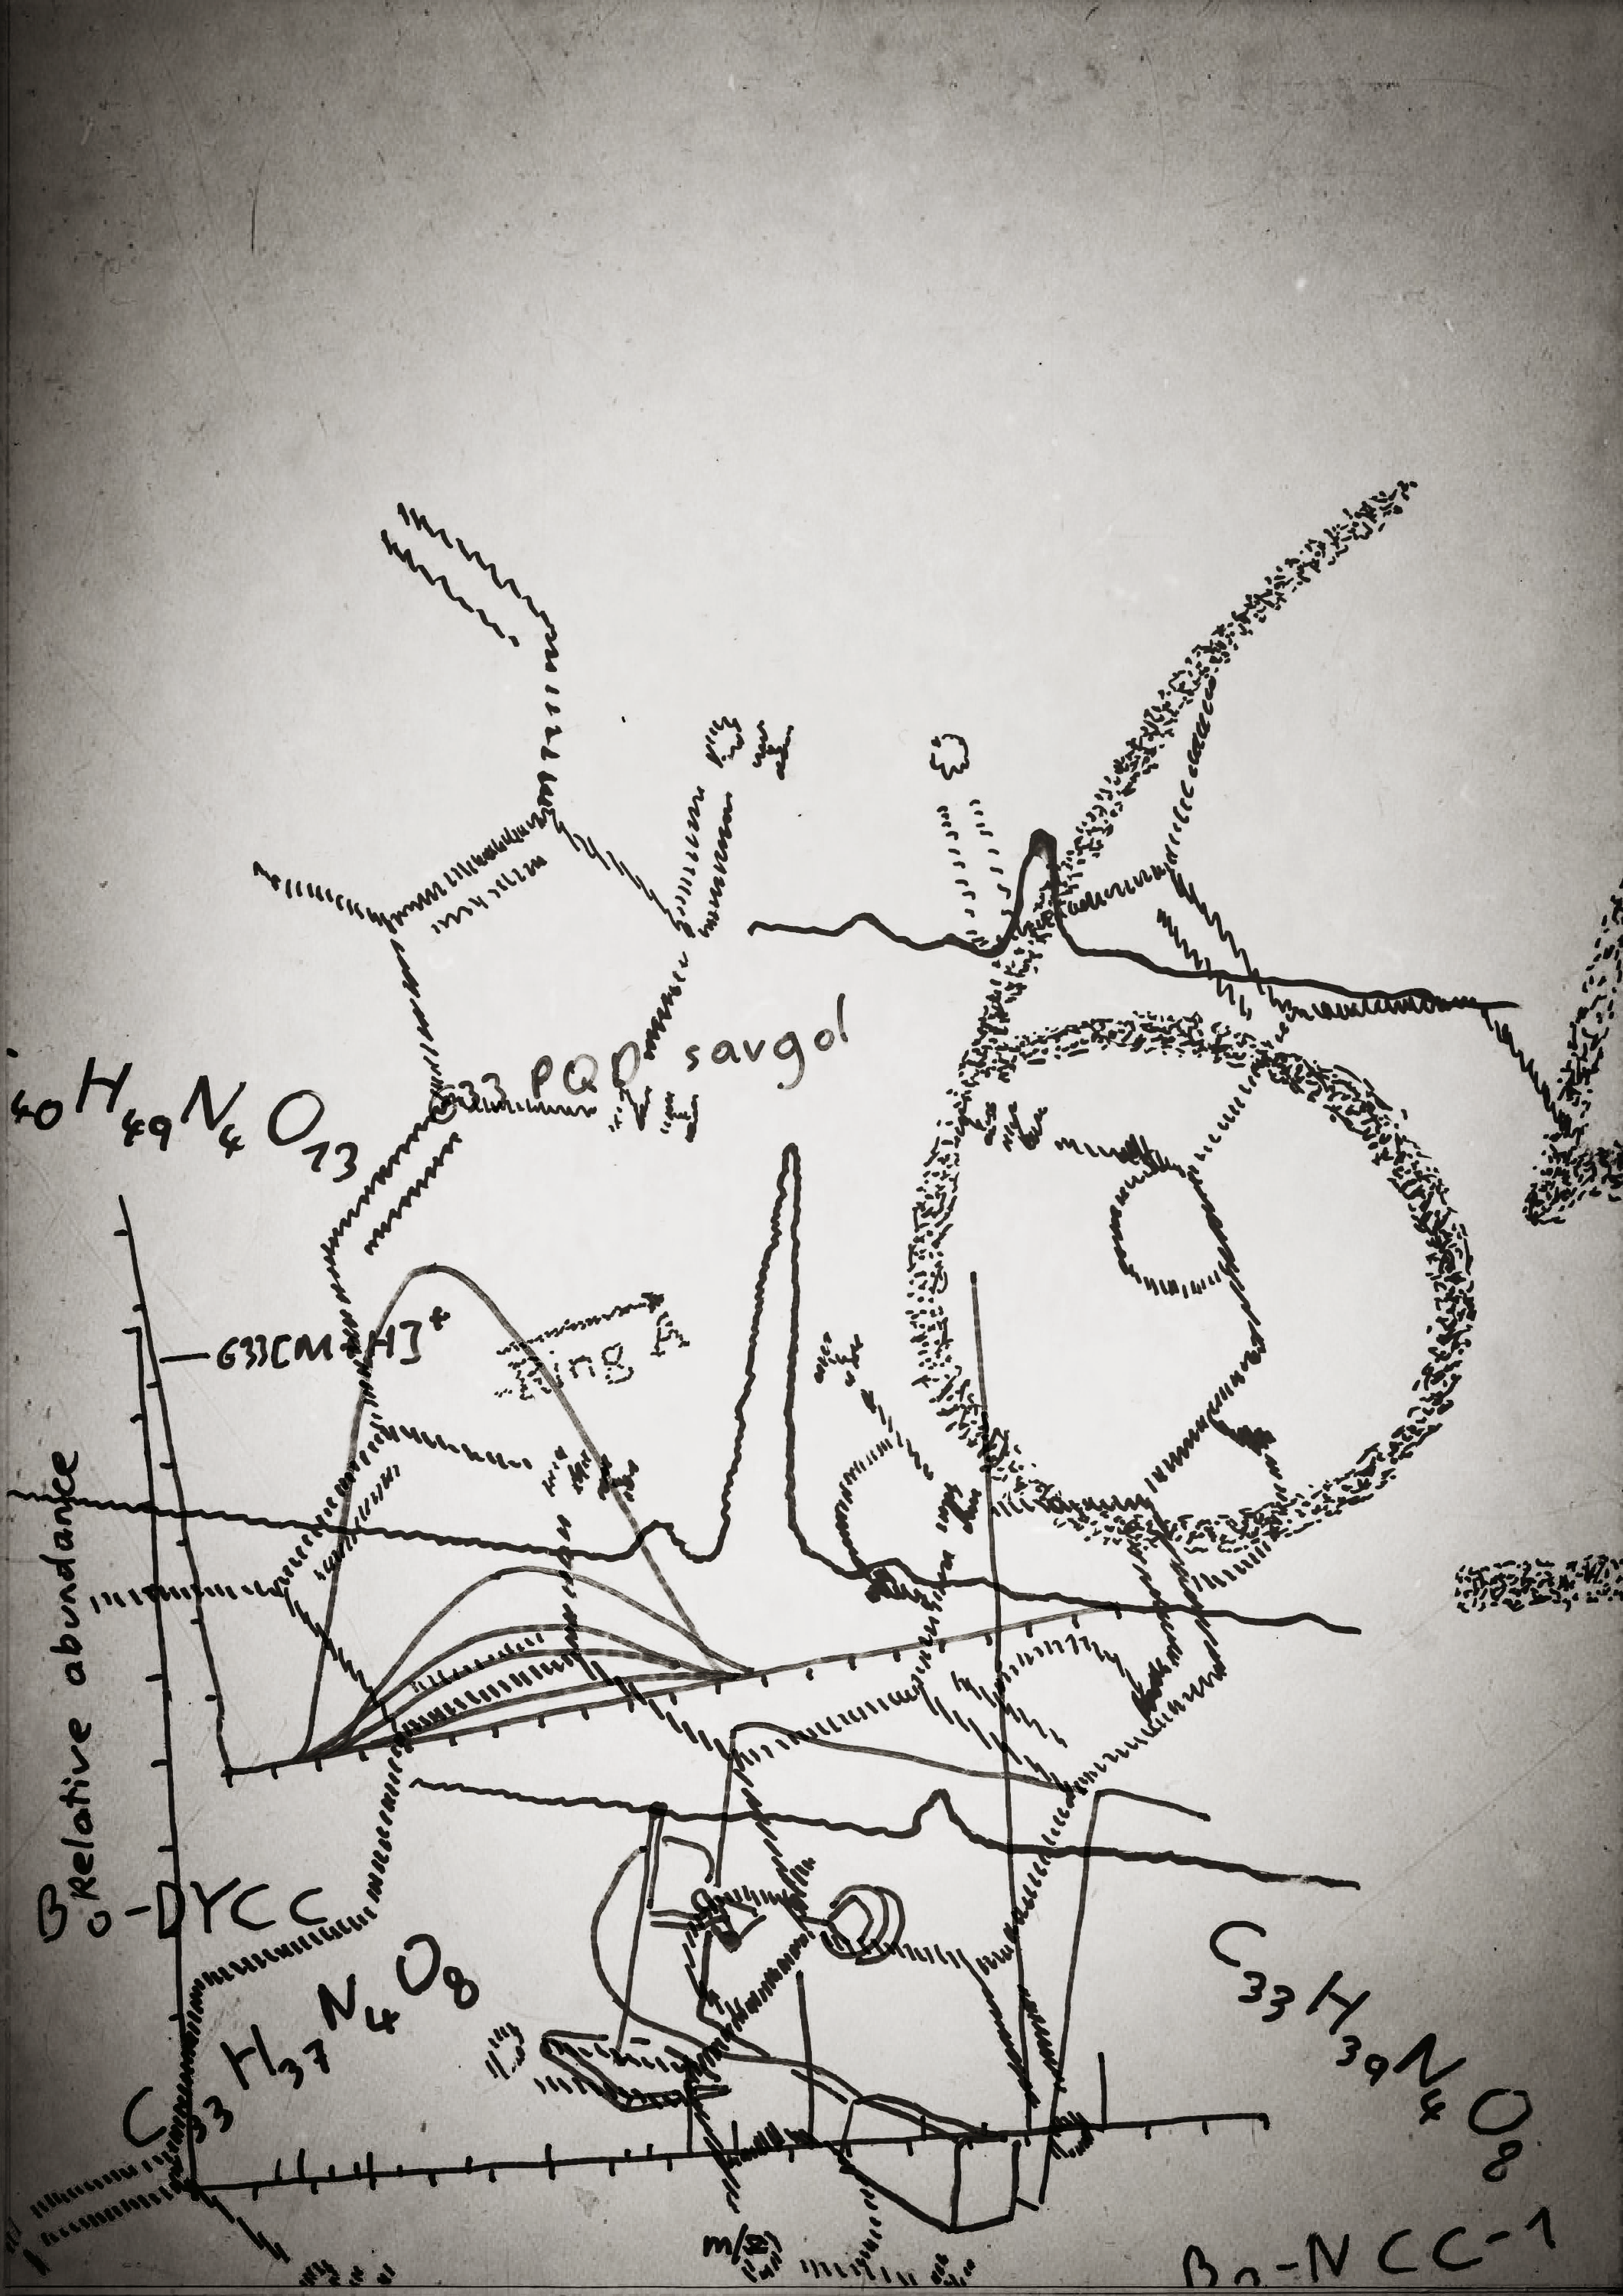
\includegraphics[width=\paperwidth,height=\paperheight]{template/VWA_Titelblatt_selected.png}%
    };
  \end{tikzpicture}
  
\cleardoublepage{}

%%%% Time-stamp: <2013-03-18 14:35:00 vk>
%% ========================================================================
%%%% Disclaimer
%% ========================================================================
%%
%% created by
%%
%%      Karl Voit


\newcommand{\mycolophon}{%%
  Diese Arbeit wurde mit \myacro{GNU}~Emacs geschrieben, in
  Palatino mit Hilfe von \href{http://LaTeX.TUGraz.at}{pdf\LaTeX2e} und
  \href{http://en.wikipedia.org/wiki/Biber_(LaTeX)}{\texttt{Biber}} gesetzt.

  Die \LaTeX{} Vorlage von Karl Voit basiert auf
  \href{http://www.komascript.de/}{KOMA script} und steht im Internet
  zum Download bereit: \href{https://github.com/novoid/LaTeX-KOMA-template}{https://github.com/novoid/LaTeX-KOMA-template}
}


%%% Local Variables: 
%%% mode: latex
%%% mode: auto-fill
%%% mode: flyspell
%%% eval: (ispell-change-dictionary "en_US")
%%% TeX-master: "../main"
%%% End: 
                %% defines information about editor, LaTeX, font, ...

%% Choose your desired title page:
\input{\mytitlepage}            %% include title page


%\input{template/declaration_TU_Graz}  %% Statutory Declaration
% \input{thanks}                %% this is a suggestion: you have to create this file on demand
% \input{foreword}              %% this is a suggestion: you have to create this file on demand


%% include the abstract without chapter number but include it on table of contents:
\cleardoublepage
%\phantomsection
\addcontentsline{toc}{chapter}{Abstract}
%%%% Time-stamp: <2013-02-25 10:31:01 vk>

\pagenumbering{gobble}

\chapter*{Abstract}
\label{cha:abstract}

Chlorophyllkataboliten sind die Endprodukte des Abbauprozesses von Chlorophyll. Im Rahmen eines Praktikums am Organischen Institut der Universität Innsbruck wurden die Chl-Kataboliten frischer Brokkoliblätter einer direkten Analyse mit MS Leafspray unterzogen. 

MS Leafspray stellt dabei eine neue Methode der Massenspektrometrie dar, die es ermöglicht, Probenmaterial in natürlicher Umgebung zu analysieren. Nach einer Erstidentifikation über MS Leafspray wurde das Ergebnis mit LC-MS verifiziert. Die mit beiden Methoden gefundenen Chl-Kataboliten lauten wie folgt: Bo-NCC-1, Bo-NCC-3, Bo-DNCC, Bo-DNCC-2, Bo-DYCC und Bo-YCC. Im Vergleich zum Brokkoliblatt konnten 4 weitere Chl-Kataboliten gefunden werden, was neue Fragen in Bezug auf das Verständnis des Abbauprozesses aufwirft. Für jeden der genannten Chl-Kataboliten konnten Strukturvorschläge gemacht werden, die noch mit \textsuperscript{1}H-NMR überprüft werden müssten.

Außerdem wurde eine Reaktion am Blatt der Chl-Kataboliten mit Essigsäureanhydrid durchgeführt. Die Reaktionsprodukte (Anhydride) konnten mit MS Leafspray durch die Beobachtung einer Massenzunahme nachgewiesen werden. Auf Basis diverser Fragmentierungen wird vorgeschlagen, dass die Reaktion nur an einer der beiden freien Carbonsäuren der Chl-Kataboliten erfolgt. 

Im Rahmen der massenspektrometrischen Analysen wurden Fragmentierungsdiagramme erstellt, von denen angesichts der Ergebnisse vermutet wird, dass sie charakteristisch für bestimmte Chl-Kataboliten sind. Eine Interpretationsmöglichkeit der Diagramme konnte vorgeschlagen werden. 

Es wurde somit ein wesentlicher Beitrag zur Weiterentwicklung der direkten Analyse mit MS Leafspray geleistet sowie konnte diese Methode mit der klassischen LC-MS verglichen werden. Zudem wurde ein Grundstein für die weitere Erforschung von Fragmentierungsdiagrammen und ihrer Aussagekraft gelegt. Zu guter Letzt konnte einiges zum Verständnis der Durchführung einer Reaktion mit Essigsäureanhydrid beigetragen werden.



%\glsresetall %% all glossary entries should be used in long form (again)
%% vim:foldmethod=expr
%% vim:fde=getline(v\:lnum)=~'^%%%%\ .\\+'?'>1'\:'='
%%% Local Variables:
%%% mode: latex
%%% mode: auto-fill
%%% mode: flyspell
%%% eval: (ispell-change-dictionary "en_US")
%%% TeX-master: "main"
%%% End:
              %% Abstract

\cleardoublepage
%\phantomsection
\addcontentsline{toc}{chapter}{Vorwort und Danksagung}
\chapter*{Vorwort und Danksagung}
\label{cha:Vorwort}

\begin{quotation}
\glqq Als ich vierzehn war, war mein Vater so unwissend. Ich konnte den alten Mann kaum in meiner Nähe ertragen. Aber mit einundzwanzig war ich verblüfft, wieviel er in sieben Jahren dazugelernt hatte.\grqq - Mark Twain
\end{quotation}

Im Rückblick auf meine VWA bin ich froh, dieses Forschungsthema gewählt zu haben. Der Wissensgewinn, den ich dabei erfahren konnte ist ungefähr so groß, wie der im Zitat beschriebene\footnote{obwohl ich nicht einundzwanzig bin}. Auch wenn die Auseinandersetzung mit diesem Thema nicht immer leicht war, machte es unheimlich viel Spaß, sich mit Fragestellungen in Form von Experimenten und deren Analyse zu beschäftigen, mit dem Ziel, ein solides Verständnis des Forschungsobjektes zu erlangen.\\

Die eingehendere Beschäftigung mit diesem Thema ermöglichte ein Praktikum im Rahmen des \textit{Sparkling Science} Projektes am Institut für Organische Chemie Innsbruck, das ich im August 2017 absolvieren durfte. Betreut wurde ich dabei von Herrn Dr. Thomas Müller, dem ich an dieser Stelle einen großen Dank für seine Geduld und die vielen Ratschläge aussprechen möchte. Er führte mich in alle für die Analyse von Chl-Kataboliten notwendigen Arbeiten ein und zeigte mir so zum Beispiel, wie ein Massenspektrometer, eine HPLC oder ein Exikator bedient werden. In der zweiten Woche konnte ich bereits selbständig operieren und die Experimente (fast) ganz nach meinen Wünschen planen und durchführen. 

Die Besprechung und Diskussion der Ergebnisse war selbstverständlich ebenso Teil der täglichen Praxis und es machte mir ungeheuer viel Spaß, meine geglaubten Erkenntnisse\footnote{im Gespräch erwies es sich des öfteren, dass ich mich etwas vertan hatte} zu besprechen und mitzuteilen. So konnte ich Einblick in andere Denkweisen gewinnen und bekam immer wieder Publikationen zum Lesen von Herrn Müller, die mir Denkanstöße und Impulse für weitere Analysen gaben. Auf diese Weise wurde ich zum Beispiel auf die Möglichkeit der Erstellung von Fragmentierungsdiagrammen aufmerksam. 

Ich denke, ich werde mich an diese Zeit noch lange zurückerinnern können, da ich dabei viel in puncto Zeitmanagement, Planung und dem generellen Ablauf des Forschungsalltags an sich erfahren konnte. Mein Wunsch, eines Tages nach einem erfolgreich absolviertem Studium der Naturwissenschaften in der Forschung tätig zu sein, wurde in dieser Zeit bestärkt. Mir gefällt einfach der Blick auf die Natur aus einer forschungstechnischen Perspektive heraus, was ich auch versuche, in dieser Arbeit ersichtlich zu machen.\\

Mein weiterer Dank ist an meinen Betreuungslehrer Mag. Mathias Scherl gerichtet. Er schaffte es in der 5ten Klasse, mein Interesse an der Chemie zu wecken, dessen Effekt bis heute ungebremst anhält. Durch ihn wurde ich erst auf die Möglichkeit des Praktikums hingewiesen und mein Interesse an der Erforschung des Abbauprozesses von Chlorophyll geweckt. Zusätzlich steht er immer für chemiespezifische Fragen bereit, was ich sehr schätze und durch deren Diskussion ich viel gelernt habe und noch lerne. 

Ansonsten möchte ich mich bei allen weiteren beteiligten Personen bedanken, die in irgendeinster Weise bei der Verfassung dieser Arbeit von Hilfe waren\footnote{ein großer Dank gilt meiner Familie und Freunden}. Insbesondere seien hier Stefanie ... und Karian genannt, ebenfalls vom Organischen Institut, die mich während des Praktikums betreuten.  

Zu guter Letzt möchte ich mich bei den Brokkoliblättern aus dem Garten meiner Oma bedanken. Ohne dieses wahrhaftig erstklassige Forschungsobjekt wäre ich unter Umständen zu gar keinem Ergebnis gekommen. Ihr wart ein wahrer Glücksgriff - DANKE! \\

Es hat mir somit das Beschäftigen mit diesem Thema sehr viel Freude bereitet. Das Ergebnis meiner Bemühungen soll in der vorliegenden Arbeit ersichtlich werden. Zu meiner Motivation zum Experimentieren an sich: \\

\begin{quotation}
 \glqq It is well to remember that most arguments in favor of not trying an experiment are too flimsily based.\grqq - R.B. Woodward
 \end{quotation} 

              %% Abstract

\pagenumbering{gobble}
\tableofcontents                %% this produces the table of contents - you might have guessed :-)


%% if myaddlistoftodos is set to "true", the current list of open todos is added:
\ifthenelse{\boolean{myaddlistoftodos}}{
  \newpage\listoftodos          %% handy if you are using todonotes with \todo{}
}{}                             %% with todonotes-package option "disable" you can get rid of any todo in the output

%\mainmatter                     %% KOMA: marks main part using arabic page numbers and such; only available in scrbook

\cleardoublepage
% \phantomsection
\pagenumbering{arabic} 
\addpart{Allgemeiner Teil}


\chapter{Themenstellung} \label{sec:Themenstellung}

Das Ziel der vorliegenden Arbeit besteht darin, die \gls{Chl-K} von Brokkoliblättern einer direkten massenspektrometrischen Analyse zu unterziehen und sie anhand unterschiedlicher Merkmale zu untersuchen.

Es sollte dabei untersucht werden, inwieweit eine direkte Analyse mit der modernen Methode MS-Leafspray eine strukturelle Aufklärung von \gls{Chl-K}en ermöglicht sowie, ob das Stattfinden einer Reaktion von Essigsäureanhydrid mit den \gls{Chl-K}en festgestellt werden kann. 

Als Ergebnisse der Reaktion werden Anhydride als Reaktionsprodukte sowie ein Verständnis über die Reaktivitäten von Carbonsäuren der \gls{Chl-K}en und deren struktureller Besonderheiten erwartet.\\

Mithilfe von im \gls{cid} Modus erstellten Fragmentierungsdiagrammen wird versucht, charakteristische Eigenschaften der \gls{Chl-K}en ausfindig zu machen. Diese Eigenschaften können sich z. B. im Vergleich der aufgenommenen Diagramme zwischen den \gls{Chl-K}en oder im intramolekularen Bereich ergeben. 

Es soll somit das Potential von Fragmentierungsdiagrammen mit Hinblick auf zukünftige Strukturaufklärung mithilfe eines Massenspektrometers analysiert werden. \\

Um die Ergebnisse von MS-Leafspray zu überprüfen wurde die Methode der \gls{hplc} sowie ein hochauflösendes Massenspektrometer verwendet. Mit den im hochauflösenden Massenspektrometer erhaltenen Fragmentierungen wird versucht, diese mit jenen von MS-Leafspray zu vergleichen, um einen Vergleich der beiden Methoden anstellen zu können.





   %% remove this line to get rid of the example chapter
\chapter{Das Chlorophyll und sein Abbauprozess}

\section{Der Abbauprozess und seine Bedeutung}

Jedes Jahr werden weltweit schätzungsweise $10^{9}$ Tonnen an Chlorophyll abgebaut. Der Abbauprozess des Chlorophylls ist damit aufgrund der markanten Farbveränderungen einer der visuell am meisten wahrgenommenen biochemischen Vorgänge und kann sogar aus dem All beobachtet werden. \cite{ChlorophyllBreakdown} Die schönen, bunten Farben des Herbstlaubes werden dabei jedoch nicht primär durch die Abbauprodukte des Chlorophylls (im Folgenden Chlorophyll-Kataboliten) hervorgerufen  \cite{DegradationChlorophyll}, da die Endprodukte des Chlorophyllabbaus zumeist farbblos sind. \cite{ChlorophyllBreakdown} Im Folgenden ist immer die Rede vom Abbauprozess in höheren Pflanzen, da gezeigt wurde, dass z. B. marine Lebensformen das Chlorophyll auf einem anderen Wege abbauen und dementsprechend andere Endprodukte vorzufinden sind. \cite{ChlorophyllBreakdown}, \cite{ErsterKatabolit}, \cite{ChlorophyllCataboliteDifferent} Die Abbauprodukte fallen in die Klasse der Phyllobiline (heterocyclische Tetrapyrrole) und sind Anzeichen für Reifung, Seneszenz und Zelltod. Der Abbauprozess wird unter anderem im Rahmen eines Entgiftungsprozesses begangen. \cite{ChlorophyllKatabolitenalsZeichenReifung}

\begin{figure}[!hbtp]
  \centering
  \includegraphics[scale=0.5]{figures/Kapitel2/VWA_Schema_Chlorophyllabbau.png}
  \caption[Abbauprozess des Chlorophylls, Quelle: http://www.organische-chemie.ch/chemie/2007nov/antioxidantien.shtm (Zugegriffen am: 05.11.2017)]{Abbauprozess des Chlorophylls in seneszenten Blättern}
  \label{fig:Chlorophyllabbau}
\end{figure}

Die Struktur eines \gls{Chl-K}en konnte erstmalig im Jahre 1991 aufgeklärt werden. Es handelte sich hierbei um einen \textit{Hv}-NCC der Gerste (\textit{Hordeum vulgare}) \cite{ErsterKatabolit}, das Endprodukt eines mehrstufigen Abbauprozesses. 

In den darauffolgenden Jahren fand man heraus, dass das Chlorophyll zuerst in das Pheophorbid a umgewandelt wird. Im nächsten Schritt wird der Makrozyklus oxygenolytisch (an der Reaktion beteiligtes Enzym: Pheo \textit{a} Mono-oxygenase \cite{ChlorophyllCatabolitesEnzyme}) in der nördlichen \textit{meso} Position geöffnet, woraufhin ein \textit{Red Chlorophyll Catabolite} (RCC) entsteht. 
Über einen \textit{primary flourescent Chlorophyll Catabolite} (pFCC) entsteht durch eine nichtenzymatische Isomerisierung ein \gls{NCC}. Thermodynamische Triebkraft dieser Reaktion ist die Rearomatisierung von Ring D. \cite{FCCKatabolit}, \cite{ChlorophyllCatabolites} Die unterschiedlichen Arten von \gls{NCC}s ergeben sich durch Anlagerung der entsprechenden funktionellen Gruppen (z. B. Zuckerring, Hydroxygruppe) an den pFCC. \cite{ChlorophyllCatabolites} 

\section{Nummerierung von Phyllobilinen}

\begin{figure}[!hbtp]
  \centering
  \includegraphics[scale=0.61]{figures/Kapitel2/VWA_Chl-Nummerierung.png}
  \caption[Nummerierung von Phyllobilinen, Quelle: Mathias Scherl]{Positionsangaben und Bezeichnungen der Ringe, die in der restlichen Arbeit für Ausführungen verwendet werden.}
  \label{fig:NummerierungPhyllobiline}
\end{figure}




\chapter{Methoden}

Es folgen theoretische Erklärungen der Methoden, derer ich mich im Rahmen meiner praktischen Arbeit bediente.

\section{HPLC}

Die \gls{hplc} ist eine chromatograpische Methode, um lösliche Stoffe präparativ zu trennen. Es sind dabei quantitative und qualitative Analysen möglich. \cite[S. 165]{Chromatographie} 

Das Trennen der Stoffe basiert auf ihren unterschiedlichen chemischen Eigenschaften. Die Stoffe werden gelöst und bilden zusammen mit dem \gls{lm} die mobile Phase, die an einer, sich in der Trennsäule befindenden stationären Phase vorbeiströmt, wobei es dabei zu Wechselwirkungen zwischen den gelösten Stoffen mit der stationären Phase kommt. Aufgrund der unterschiedlichen chemischen Eigenschaften und den daraus resultierenden unterschiedlichen Wechselwirkungen hält sich jeder Stoff verschieden lange in der stationären Phase auf. Die Verweildauer eines Stoffes in der Trennsäule wird als Retentionszeit bezeichnet. \cite[S. 31-32]{Chromatographie} Die Retentionszeit wird über Detektoren bestimmt, die die Änderung der Zusammensetzung der mobilen Phase feststellen und das Ergebnis in einem Chromatogramm darstellen. \cite[S. 46]{Chromatographie} 

Für die Experimente wurde die Methode der \gls{rp} Chromatographie angewandt. Dabei ist die mobile Phase polar und die stationäre Phase unpolar (als unpolare Phase dienen beispielsweise Silane mit langen Kohlenwasserstoffketten). \cite[S. 189]{Chromatographie}\\

Im Rahmen meiner Arbeit wurde die \gls{hplc} verwendet, um die Stoffe im Blatt zu trennen und entsprechende \gls{Chl-K}en zu isolieren. Die Identifikation der \gls{Chl-K}en erfolgte dabei durch einen UV/VIS Detektor (operierte im Wellenlängenbereich von 200nm - 800nm) sowie durch ein dazu geschaltetes Massenspektrometer (=\gls{lcms}). Um die \gls{Chl-K}en mit einem hochauflösenden Massenspektrometer zu fragmentieren, wurden die Verbindungen zu jenen Zeiten, zu denen sie in der \gls{hplc} jeweils eluieren in \gls{eppi} gesammelt.\\

Die Herstellung eines Blattextraktes für die Analyse mit der \gls{hplc} wird in Kapitel \ref{sec:HPLCAufarbeitungderProbe} beschrieben. Aufgrund dieser speziellen Aufarbeitung des Blattes zählt die Methode der \gls{hplc} nicht mehr zur direkten Analyse. Sie wurde lediglich verwendet, um die Ergebnisse von MS Leafspray zu verifizieren.

\section{Massenspektrometrie}

Mithilfe eines Massenspektrometers kann die Masse eines Moleküls bestimmt werden. Aufgrund der Einfachheit der Methode und der sehr geringen benötigten Probenmenge ist das Massenspektrometer für eine Vielzahl an Anwendungen geeignet (\gls{zB} in der Forensik, Lebensmittelprüfung, Medikamentenprüfung, Analyse von Meteoriten). \cite[S. 1]{MassSpectrometry} Der jetzige Entwicklungsstand in der Massenspektrometrie ist vor allem den Entwicklungen der letzten vier Jahrzehnte zu verdanken. \cite[S. 6-9]{MassSpectrometry} \\

Um die Molekülmasse der Stoffe zu bestimmen, werden sie zuerst in Gasphasen-Ionen überführt. \cite[S. 15]{MassSpectrometry} Dabei gibt es unterschiedliche Methoden, diesen Zustand herbeizuführen, wie \gls{zB} Electron Ionization, Chemical Ionization und Field Ionization. \cite[S. 15-30]{MassSpectrometry} Nach der Ionisation werden sie im Massenanalysator nach ihrem \gls{mz} Verhältnis getrennt und im Detektor der Ionenstrom gemessen. Das Ergebnis wird in einem Massenspektrum festgehalten, in dem auf der Ordinate die relative Intensität der einzelnen Peaks und auf der Absizze das Verhältnis \gls{mz} aufgetragen werden. \\

In den Experimenten dieser Arbeit wurde zur Ionisation die \gls{ESI} Methode verwendet, die erstmalig das Messen von Proteinen mithilfe eines Massenspektrometers erlaubte und aufgrund ihrer hohen Empfindlichkeit gegenüber kleinen, polaren Molekülen mit einer \gls{hplc} kombiniert werden kann. Bei der \gls{ESI} Methode wird durch Anlegen einer Spannung von 3-6kV zwischen der Kapillare, aus der die Flüssigkeit kommt und der Gegenelektrode ein elektrisches Feld mit einer Stärke in der Größenordnung von $10^{6}$ $Vm^{-1}$ angelegt. Die erhaltenen geladenen Tröpfchen passieren ein Inertgas (in den meisten Fällen \gls{n2}) \gls{bzw} eine erhitzte Kapillare, um das \gls{lm} zu entfernen. Anschließend an diese Ionisation wird die Molekülmasse der Ionen bestimmt. \cite[S. 43-44]{MassSpectrometry} \\

Um die Chlorophyllkataboliten im Massenspektrometer zu analysieren, wurde sowohl die Methode der \gls{lcms} als auch die Methode des MS-Leafspray verwendet. 

\subsection{LC-MS}

Bei der Methode der LC-MS wird eine \gls{hplc} vor ein Massenspektrometer geschaltet. Dabei trennt die \gls{hplc} die Stoffe zuvor auf und eluiert sie anschließend in das Massenspektrometer. \cite[S. 217-218]{MassSpectrometry} Um die Flussrate bei atmosphärischem Druck zu verringern, wird nur ein Teil des direkt aus der \gls{hplc} kommenden Flusses zum Massenspektrometer hin abgezweigt. Ansonsten wäre die Flussrate zu hoch, was eine Ionisierung der Probe mithilfe einer \gls{ESI} - Quelle unmöglich machen würde. \cite[S. 221]{MassSpectrometry} 

Das Resultat ist je ein Chromatogramm der HPLC und des Massenspektrometers. Es wird somit zu jedem Zeitpunkt eines \gls{hplc}-Laufes ein UV/VIS Spektrum sowie ein Massenspektrum erzeugt. Aus dem UV/VIS Spektrum lässt sich schließen, ob es sich bei einem \gls{Chl-K}en um einen \gls{NCC}, \gls{DNCC} oder einen \gls{YCC} handelt. Aus dem Massenspektrum kann die Molekülmasse (in Da) mit allgegenwärtigen Fragmentierungen abgelesen werden. Unter Verwendung eines hochauflösenden Massenspektrometers wird außerdem die atomare Zusammensetzung in Form einer Summenformel ersichtlich. \\

\subsection{MS Leafspray} \label{sec:MSLeafspray}

\textit{Ambient Ionization} \cite{AmbientIonisation} ermöglicht es, Proben ohne vorherige präparative Trennung durch chromatographische Trennverfahren direkt in ihrer \textit{natürlichen} Umgebung mithilfe eines Massenspektrometers zu untersuchen. Eine Methode, die auf dem Prinzip der \textit{Ambient Ionization} basiert ist \textit{Paper Spray} \cite{PaperSpray}. Dabei  kommt es zu einer Kombination der \gls{ESI} sowie der \textit{Ambient} Ionisationsmethode. \cite{PaperSpray}\\

Die Ionisation der Probe erfolgt ausgehend von einem feuchten, porösen Material (\gls{zB} Papier), das in einer Kupferklemme eingeklemmt wird. Zwischen der Kapillaröffnung des Massenspektrometers und der Kupferklemme liegt eine Spannung im Bereich von 3-6kV an, woraufhin kleine Tröpfchen, die Ionen der Probe enthalten von der Spitze des porösen Materials ausgesendet werden und Ionen der Probe in das Massenspektrometer befördern. \cite{RapidScreeningLeafSpray} Durch Anlegen von Kalibrationskurven mit externen Standards wird außerdem ermöglicht, eine quantitative Bestimmung der Menge des Analyten durchzuführen. \cite{LeafSpray}

Leaf Spray ist eine Form von Paper Spray, bei der die zu analysierende Pflanze selbst als poröses Material dient. Sie wurde im Rahmen dieser Arbeit für die Identifikation von \gls{Chl-K}en verwendet. Ein Vorteil einer Analyse von \gls{Chl-K}en mit MS Leafspray ist, dass weniger Zeit für die Vorbereitung benötigt wird, was wiederum Grundlage für eine schnellere und effizientere Analyse ist. Genauere Ausführungen zur Durchführung finden sich in Kapitel \ref{sec:MSLeafspray}.\\



\addpart{Experimenteller Teil}

\chapter{Allgemeine Arbeits- und Analysemethoden}

\section{Herstellung von Lösungen für eine Analyse mit HPLC}

\section{Fragmentierungsdiagramme} \label{sec:fragmentierungsdiagramme}

Zu jedem Kataboliten wurde ein Fragmentierungsdiagramm erstellt. Dazu werden die Intensitäten der einzelnen beobachteten Fragmentierungen im Massenspektrometer zur aufgewendeten, normaliserten Kollisionsenergie (alle fünf Einheitsschritte) aufgenommen. Auf der Abszisse des erhaltenen Diagramms befindet sich die normalisierte Kollisionsergie in Prozent und auf der Ordinate die Intensität der einzelnen bezogen auf den höchsten Peak, der während der Aufnahme beobachtet wurde, in Prozent. Die erhaltenen Kurven wurden mit einem Savitzky-Golay Filter geglättet (siehe Anhang) und werden im folgenden als Fragmentierungsdiagramme bezeichnet. Ein Nachteil bei der Behandlung mit diesem Filter ist, dass in manchen Fällen die Graphen der Fragmentierungen bei einer normalisierten Kollisionsenergie von null nicht null sind. Es wird im folgenden angenommen, dass dies dennoch so ist.

Die Fragmentierungsdiagramme wurden sowohl im \gls{cid} als auch im \gls{pqd} Modus aufgenommen. 

Es wird damit versucht, herauszufinden, ob bestimmte Abspaltungen der Kataboliten charakteristische Muster aufweisen, um in weiterer Hinsicht, weitere strukturelle Eigenschaften über die Kataboliten mithilfe eines Massenspektrometers zu erfahren. Weiters wird ein Vergleich zwischen den Fragmentierungsdiagrammen von MS Leafspray und des hochauflösenden Massenspektrometers versucht. Für diesen Vergleich wurden nur die Diagramme verwendet, die im \gls{cid} Modus aufgenommen wurden, da das verwendete Massenspektrometer von MS Leafspray nur in diesem Modus operieren konnte.
\chapter{Experimente MS-Leafspray} \label{sec:MSLeafspray}

\section{Gerätebeschreibung Massenspektrometer}

(Beschreibung Massenspektrometer)

\section{Versuchsaufbau} \label{sec:Versuchsaufbau}

Abbildung \ref{fig:LeafsprayVersuchsaufbau} beschreibt schematisch den Versuchsaufbau. 

\begin{figure}[!hbtp]
  \centering
  \includegraphics[scale=0.5]{figures/Kapitel4/VWA_MSLeafspray_Versuchsaufbau.png}
  \caption[MS-Leafspray Versuchsaufbau, Quelle: Autor]{Leafspray Versuchsaufbau: 1) Filterpapierdreick, 2) Spitze des Dreiecks, 3) Blattmaterial, von Filterpapier umschlossen, 4) Kupferklemme, 5) Kapillare für \gls{lm}, 6) Einlass des Massenspektrometers (mit der markanten Spitze zwecks Verdeutlichung etwas übertrieben dargestellt), 7) \textit{Syringe Pump} - kontrolliert den \gls{lm}-Fluss durch 5), 8) DESI Massenspektrometer, 9) Stativ, 10) Kabel, mit 4) verbunden - zwischen 4) und 6) liegt eine Spannung   an (3-6kV - durch Blitz zwischen 2) und 6) symbolisiert)}
  \label{fig:LeafsprayVersuchsaufbau}
\end{figure}

Das zu analysierende Blatt wurde zugeschnitten und in Filterpapier eingerollt. Das Filterpapierdreieck wurde in einer Kupferklemme eingespannt (Kapitel \ref{sec:Versuchsdurchfuehrung}). Die Kupferklemme wurde mit einem Kabel (10), das an einem DESI-Massenspektrometer (8) angeschlossen war, verbunden. Zwischen der Kupferklemme (4) und dem Massenspektrometer wurde eine Spannung von 3-6kV angelegt. Da das Filterpapier mit \gls{lm} benetzt ist und eine Verbindung der Flüssigkeit zur Kupferklemme besteht, kommt es zu einer durch die Spannung ausgelösten Bewegung der im \gls{lm} gelösten Ionen, die nun in das Massenspektrometer hineinfliegen. Der Abstand zwischen Filterpapier (2) und Einlass des Massenspektrometers (6) betrug ungefähr 0.5cm und ist damit der Flugstrecke der Ionen gleichzusetzen. 

\begin{figure}[htbp]
  \begin{subfigure}[b]{0.5\textwidth}
    \includegraphics[width=\textwidth]{figures/Kapitel4/VWA_MSLeafspray_Detail1.jpg}
    \caption{}
    \label{fig:MSLeafsprayDetail1}
  \end{subfigure}
  \hfill
  \begin{subfigure}[b]{0.5\textwidth}
    \includegraphics[width=\textwidth]{figures/Kapitel4/VWA_MSLeafspray_Detail2.jpg}
    \caption{}
    \label{fig:MSLeafsprayDetail2}
  \end{subfigure}
  \caption[MS-Leafspray Versuchsaufbau Detailfotos, Quelle: Autor]{(a) Einlass des Massenspektrometers mit Kapillare, Kupferklemme und Filterpapier mit Blattmaterial, (b) Detailansicht}
  \label{fig:MSLeafsprayDetail}
\end{figure}

In Abbildung \ref{fig:MSLeafsprayDetail} wird gezeigt, wie diese Anordnung umgesetzt wurde. Zu sehen sind die Kupferklemme mit dem eingespannten Filterpapier und dem darin enthaltenen Blatt, die \gls{lm}-Kapillare, die Einlassöffnung des Massenspektrometers und der Abstand von Filterpapierdreicksspitze zum Massenspektrometer. Es gilt zu beachten, dass das Blatt in einem gewissen Winkel eingespannt wird, um zu verhindern, dass das \gls{lm} nicht abfließt, was bei einer waagrechten Anordnung auftreten kann (Abbildung \ref{fig:MSLeafsprayDetail2}). 

\section{Versuchsdurchführung} \label{sec:Versuchsdurchfuehrung}

Frische, seneszente Brokkoliblätter und Filterpapier wurden mit Rasierklinge und Schere wie in Abbildung \ref{fig:LeafsprayVorbereitung}a ersichtlich zugeschnitten. Anschließend wurde das Brokkoliblatt auf das Filterpapier gelegt und dieses bis zur Basis des Dreiecks eingerollt. 

Diese Art der Vorbereitung zeigte sich als besonders effektiv, da mit ihr höhere Intensitäten der Signale im Massenspektrometer erreicht werden konnten, wie wenn nur das Blatt zu einem Dreieck zugeschnitten und in dieser Form vor das Massenspektrometer gehalten wird. Grund dafür ist vermutlich, dass das \gls{lm} mehr Zeit hat, die Chlorophyllkataboliten aus dem Blatt heraus zu lösen und dass mehr Blattmaterial vorhanden ist. Außerdem behält das Filterpapier länger seine Steifigkeit wie ein Brokkoliblatt, weswegen längere Analysen mit konstanterem Signal möglich sind.

\begin{figure}[hbtp]
  \centering
  \includegraphics[scale=0.5]{figures/Kapitel4/VWA_MSLeafspray_Blattvobereitung_zwei.png}
  \caption[MS-Leafspray Blattvorbereitung, Quelle: Autor]{Leafspray Blattvorbereitung: (a) zugeschnittenes Filterpapierdreieck, mit frischen, seneszenten Brokkoliblättern, (b) eingerolltes \textit{Päckchen}, in Kuperklemme eingespannt}
  \label{fig:LeafsprayVorbereitung}
\end{figure}

Das erhaltene \textit{Päckchen} wurde durch eine Kupferklemme (Abbildung \ref{fig:LeafsprayVorbereitung}b) ca. 0.5cm  vor die Kapillare des Massenspektrometers gehalten (Abbildung \ref{fig:MSLeafsprayDetail2}). Um ein konstantes Signal zu erhalten versorgte eine Kapillare, die wie in Abbildung \ref{fig:MSLeafsprayDetail1} befestigt war, das Päckchen mit einem konstanten \gls{lm}-Fluss (als \gls{lm} wurden \gls{meoh} sowie Acetonitril verwendet). Die Flussrate des \gls{lm} betrug zu Beginn 12\si{\uL\per\minute}, um das Blatt schneller zu befeuchten und wurde ab dem Erhalt des ersten Signals auf 5\si{\uL\per\minute} zurückgefahren. Es zeigte sich, dass bei dieser Flussrate das Signal bei annähernd gleichbleibend hoher Intensität am längsten bleibt. Der Spraystrom betrug zwischen xx und xx \si{\micro\ampere}. Diese Geräteeinstellungen sowie Aufarbeitungsmethoden ermöglichten das Messen der Fragmentierungsdiagramme, da hierfür eine längere Analysezeit vonnöten ist. Das erste Signal konnte nach ca. einer Minute nach dem Einschalten der Spannung gemessen werden und erlaubte Messungen bis zu 25min. \\

\textit{(Platz für Beschreibung der Einstellungen des Gerätes)}\\

Aufgenommen wurden die Massenspektrum im Bereich von 300 \gls{mz} bis 1000 \gls{mz}, um  Massenspektren zu bekommen, die nicht so stark von anderen Ionensorten gestört werden. Gemessen wurde im positiven Ionenmodus, wobei zwischendurch in den negativen Ionenmodus gewechselt wurde, wenn die Intensität des Signals im positiven Ionenmodus abnahm. Das Wechseln des Modus konnte die gewünschte Intensität wieder erhöhen. Es wurde somit ein ähnliches Verhalten der Intensitäten im Zeitverlauf beobachtet wie in \cite{RapidScreeningLeafSpray} bereits beschrieben, wobei hier das Umschalten in den negativen Ionenmodus nicht explizit erwähnt wird, um das Problem der abnehmenden Intensitäten im positiven Ionenmodus zu beheben.

\section{Chl-Kataboliten des Brokkoliblattes mithilfe von MS-Leafspray identifiziert}

Im Folgenden werden die \gls{Chl-K}en beschrieben, die sich durch MS Leafspray identifizieren ließen. Die Strukturvorschläge wurden mit einem hochauflösendem Massenspektrometer überprüft (Kapitel \ref{sec:ChlKatabolitenBrokkoli} und \ref{sec:ChlKatabolitenESIMS}). Sie beruhen auf den exakten Molekülmassen und den daraus errechneten möglichen Summenformeln. Eine exakte Strukturaufklärung müsste mit \textsuperscript{1}H-NMR durchgeführt werden. 

Fragmentierungsdiagramme wurden wie in Kapitel \ref{sec:fragmentierungsdiagramme} beschrieben erstellt.

\subsection{Bo-NCC-1} \label{sec:MSLeafsprayBoNCC1}

Bei diesem Kataboliten handelt es sich vermutlich um denselben, wie er auch in der Brokkolifrucht gefunden wurde, weswegen er die Bezeichnugn Bo-NCC-1 erhält. \cite{ChlorophyllCatabolitesBroccoli} Beobachtet wurde die protonierte Verbindung bei m/z = 793 [M+H]\textsuperscript{+} und das Kaliumsalz bei m/z = 831 [M+K]\textsuperscript{+} (Abbildung \ref{fig:831MKLeafspray}). Aufgrund der geringen Intensitäten der protonierten Verbindung war es nicht möglich, ein verwertbares Massenspektrum dieser aufzunehmen. \\

Der Katabolit bei m/z = 831 [M+K]\textsuperscript{+} zeigte Abspaltungen von \ch{H2O} bei m/z = 813 [M - \ch{H2O} + K]\textsuperscript{+}, von \ch{CO2} bei m/z = 787 [M - \ch{CO2} + K]\textsuperscript{+} und eine Folge von Abspaltungen bei m/z = 311 [M - (Ring A, Zucker, Ring D, \ch{CO2}) + K]\textsuperscript{+}, bei der Ring A mit einem Zucker, Ring D sowie \ch{CO2} abgespalten wird (siehe Kapitel \ref{sec:ChlKatabolitenESIMS}). Die Abspaltungen bei m/z = 798 [M - (\gls{nAb}) + K]\textsuperscript{+}, m/z = 586 [M - (\gls{nAb}) + K]\textsuperscript{+} und m/z = 551 [M - (\gls{nAb}) + K]\textsuperscript{+} können nicht eindeutig zugeordnet werden, da hierzu weitere experimentelle Daten und vor allem die exakten Molekülmassen vonnöten sind. 

\begin{figure}[!htbp]
  \includegraphics[width=\textwidth, height=0.7\textwidth]{figures/Kapitel4/Kataboliten/VWA_MS_LeafSpray_831.png}
  \caption[ESI-MS Spektrum von Bo-NCC-1, Quelle: Autor]{ESI-MS von Bo-NCC-1 mit m/z = 831 [M+K]\textsuperscript{+}}
  \label{fig:831MKLeafspray}
\end{figure}

Das Fragment bei m/z = 798 [M - (\gls{meoh}?) + K]\textsuperscript{+} ist insofern interessant, da es sich hierbei um eine Abspaltung von \gls{meoh} (-32 Da) handeln könnte (es wird angenommen, dass die Abweichung um eine Einheit durch Ungenauigkeiten des Massenspektrometers zustandekommt), was aber nicht mit der Struktur des Bo-NCC-1 (siehe Abbildung \ref{fig:831MKLeafspraystructure}) vereinbar wäre. Aufgrund ihrer Fragwürdigkeit wird auf diese Abspaltung in den weiteren Ausführungen nicht näher eingegangen.

Wie aus dem Fragmentierungsdiagramm (Abbildung \ref{fig:831MKLeafspraydiags}) ersichtlich, erfolgt die Abspaltung von \ch{H2O} bei einer niedrigeren \gls{nKE} wie jene von \ch{CO2} und verschwindet bei höheren Energien, wohingegen die Abspaltung von \ch{CO2} erhalten bleibt. Die Abspaltung von \ch{H2O} erreicht ein lokales Maximum bei einer \gls{nKE} von 10. Die Abspaltung von \ch{CO2} erreicht ein lokales Maximum bei 30 \gls{nKE}.

Aufgrund der \ch{CO2} Abspaltung wird an Position 8\textsuperscript{2} eine Carbonsäuregruppe vermutet (wie in \cite{StructureElucidation} gezeigt), die über einen Mechanismus wie unter anderem (u. a.) in Abbildung \ref{fig:619MHElectronMovement} vorgeschlagen, abgespalten wird. Die relativ große Molekülmasse weist zudem auf einen Zucker an Position 32 hin. Die Summenformel des Bo-NCC-1 konnte über die exakte Molekülmasse mit einem hochauflösenden Massenspektrometer bestimmt werden (Kapitel \ref{sec:ESIMSBoNCC1}).

\begin{figure}[!htbp]
  \begin{subfigure}[b]{0.5\textwidth}
    \includegraphics[width=\textwidth]{figures/Kapitel4/Kataboliten/fragmentation_structures/VWA_Katabolit_831.png}
    \caption{}
    \label{fig:831MKLeafspraystructure}
  \end{subfigure}
  \hfill
  \begin{subfigure}[b]{0.7\textwidth}
    \includegraphics[width=\textwidth]{figures/Kapitel4/Kataboliten/diags/831CID-savgol.png}
    \caption{}
    \label{fig:831MKLeafspraydiags}
  \end{subfigure}
  \caption[Strukturvorschlag von Bo-NCC-1 und Fragmentierungsdiagramm, Quelle: Autor]{(a) Strukturvorschlag des Bo-NCC-1 mit Summenformel \ch{C40H48N4O13}, (b) Fragmentierungsdiagramm von Bo-NCC-1 (blau = 831 [M+K]\textsuperscript{+}, orange = 813 [M - \ch{H2O} + K]\textsuperscript{+}, grün = 798 [M - (\ch{MeOH} - \gls{nAb}) + K]\textsuperscript{+}, rot = 787 [M - \ch{CO2} + K]\textsuperscript{+})}
\end{figure}



\subsection{Bo-NCC-3}

Beim Bo-NCC-3 handelt es sich um einen \gls{Chl-K}, der bisher nicht in der Brokkolifrucht identifiziert wurde \cite{ChlorophyllCatabolitesBroccoli}, weswegen er als dritter, in der Brokkolipflanze gefundener Katabolit den Index 3 erhält. Analysiert wurde das Kaliumsalz mit m/z = 685 [M+K]\textsuperscript{+}. \\

Es wurden zwei charakteristische Abspaltungen von \ch{H2O} bei m/z = 667 [M - \ch{H2O} + K]\textsuperscript{+} sowie von \ch{CO2} bei m/z = 641 [M - \ch{CO2} + K]\textsuperscript{+} beobachtet. Bei den Abspaltungen bei m/z = 429 [M - (\gls{nAb}) + K]\textsuperscript{+}, m/z = 561 [M - (\gls{nAb}) + K]\textsuperscript{+}, m/z = 605 [M - (\gls{nAb}) + K]\textsuperscript{+} und m/z = 652 [M - (\gls{nAb}) + K]\textsuperscript{+} ist nicht eindeutig geklärt, welche Fragmente hierbei entstanden sind. Für das Fragment bei m/z = 652 [M - (\gls{meoh}?) + K]\textsuperscript{+} gilt dasselbe wie bei der Abspaltung von m/z = 798 [M - (\ch{MeOH}?) + K]\textsuperscript{+} von Bo-NCC-1 (Kapitel \ref{sec:MSLeafsprayBoNCC1}). Um diese Fragmente aufzuklären müssten weitere Experimente des Kaliumsalzes mit einem hochauflösenden Massenspektrometer durchgeführt werden. Fragmentierungen der protonierten Verbindung konnten mit einem hochauflösenden Massenspektrometer gemessen werden (Kapitel \ref{sec:ESIMSBoNCC3}).

\begin{figure}[htbp]
  \includegraphics[width=\textwidth, height=0.7\textwidth]{figures/Kapitel4/Kataboliten/VWA_MS_LeafSpray_685.png}
  \label{fig:685MKLeafspray}
  
  \caption[ESI-MS von Bo-NCC-3, Quelle: Autor]{ESI-MS von Bo-NCC-3 mit m/z = 685 [M+K]\textsuperscript{+}}
\end{figure}

\begin{figure}[!htbp]
  \begin{subfigure}[b]{0.4\textwidth}
    \includegraphics[width=\textwidth]{figures/Kapitel4/Kataboliten/fragmentation_structures/VWA_Katabolit_685.png}
    \caption{}
    \label{fig:685MKLeafspraystructure}
  \end{subfigure}
  \hfill
  \begin{subfigure}[b]{0.7\textwidth}
    \includegraphics[width=\textwidth]{figures/Kapitel4/Kataboliten/diags/685CID-savgol.png}
    \caption{}
    \label{fig:685MKLeafspraydiags}
  \end{subfigure}
  \caption[Strukturvorschlag von Bo-NCC-3 und Fragmentierungsdiagramm, Quelle: Autor]{(a) Strukturvorschlag von Bo-NCC-3 mit Summenformel \ch{C34H38N4O9}, (b) Fragmentierungsdiagramm von Bo-NCC-3 (blau = 685 [M+K]\textsuperscript{+}, orange = 667 [M - \ch{H2O} + K]\textsuperscript{+}, grün = 652 [M - (\gls{meoh}?) + K]\textsuperscript{+}, rot = 641 [M - \ch{CO2} + K]\textsuperscript{+}, violett = 605 [M - (\gls{nAb}) + K]\textsuperscript{+})}
\end{figure}

Das Fragmentierungsdiagramm zeigt, dass die Abspaltung von \ch{H2O} bei einer niedrigeren \gls{nKE} erfolgt, wie jene von \ch{CO2}, da sie ihre höchste Intensität zuvor erreicht (bei einer \gls{nKE} von 15 - \ch{H2O} im Vergleich zu 20 - \ch{CO2}). 

Im Vergleich zum Bo-NCC-1 zeigt der Graph ein lokales Maximum der \ch{H2O} Abspaltung bei höheren Energien (beim Bo-NCC-3 bei 15 \gls{nKE} wohingegen beim Bo-NCC-1 bereits bei 10 \gls{nKE}). Das lokale Maximum der \ch{CO2} Abspaltung verschiebt sich von 30 \gls{nKE} beim Bo-NCC-1 auf 20 \gls{nKE} beim Bo-NCC-3. Das lokale Maximum der potentiellen Abspaltung von \gls{meoh} würde sich von 25 \gls{nKE} beim Bo-NCC-1 auf 30 \gls{nKE} beim Bo-NCC-3 verschieben (Abbildungen \ref{fig:831MKLeafspraydiags} und \ref{fig:685MKLeafspraydiags}).\\ 

Wie beim Bo-NCC-1 weist die \ch{CO2} Abspaltung auf eine freie Carbonsäure an Position 8\textsuperscript{2} hin. Aufgrund der durch die Summenformel erhaltene Sauerstoffanzahl wird angenommen, dass sich an Position 15 eine Hydroxygruppe befindet (Abbildung \ref{fig:685MKLeafspraystructure}). Es wird vermutet, dass es sich dabei um eine Vorstuffe zu einem \gls{YCC} handelt. [Referenz]

\subsection{Bo-DNCC}

Es wird vermutet, dass der Bo-DNCC des Brokkoliblattes ident ist mit dem Bo-DNCC der Brokkolifrucht. \cite{ChlorophyllCatabolitesBroccoli} Beobachtet wurden zwei Pseudo-Molekulare Ionen. Eines mit m/z = 619 [M+H]\textsuperscript{+} (Abbildung \ref{fig:619MHLeafspray}) und mit m/z = 657 [M+K]\textsuperscript{+} (Abbildung \ref{fig:657MKLeafspray}).\\

Der Katabolit bei m/z = 619 [M+H]\textsuperscript{+} zeigte Abspaltungen von \ch{H2O} bei m/z = 601 [M - \ch{H2O} + H]\textsuperscript{+}, von \ch{CO2} bei m/z = 575 [M - \ch{H2O} + H]\textsuperscript{+}, von Ring D (zusammen mit einer Abspaltung von \ch{CO2}) bei m/z = 452 [M - (Ring D, \ch{CO2}) + H]\textsuperscript{+} und von Ring A, Ring D und \ch{CO2} bei m/z = 311 [M - (Ring A, Ring D, \ch{CO2}) + H]\textsuperscript{+} (Abbildung \ref{fig:619MHLeafspray} - Zuordnung Kapitel \ref{sec:ESIMSBoDNCC}).

\begin{figure}[!htbp]
  \includegraphics[width=\textwidth, height=0.7\textwidth]{figures/Kapitel4/Kataboliten/VWA_MS_LeafSpray_619.png}
  \caption[ESI-MS von Bo-DNCC, Quelle: Autor]{ESI-MS von Bo-DNCC bei m/z = 619 [M+H]\textsuperscript{+}}
  \label{fig:619MHLeafspray}
\end{figure}

Das Kaliumsalz des Bo-DNCC mit m/z = 657 [M+K]\textsuperscript{+} zeigte eindeutige Abspaltungen von \ch{H2O} bei m/z = 639 [M - \ch{H2O} + K]\textsuperscript{+} und von \ch{CO2} bei m/z = 613 [M - \ch{CO2} + K]\textsuperscript{+} (Abbildung \ref{fig:657MKLeafspray}). Die Abspaltungen bei m/z = 375 [M - (\gls{nAb}) + K]\textsuperscript{+} und m/z = 577 [M - (\gls{nAb}) + K]\textsuperscript{+} können nicht eindeutig zugeordnet werden.

\begin{figure}[!htbp]
  \includegraphics[width=\textwidth, height=0.7\textwidth]{figures/Kapitel4/Kataboliten/VWA_MS_LeafSpray_657.png}
  \caption[ESI-MS von Bo-DNCC, Quelle: Autor]{ESI-MS von Bo-DNCC bei m/z = 657 [M+K]\textsuperscript{+}}
  \label{fig:657MKLeafspray}
\end{figure}

\begin{figure}[!htbp]
  \begin{subfigure}[b]{0.4\textwidth}
    \includegraphics[width=\textwidth]{figures/Kapitel4/Kataboliten/fragmentation_structures/VWA_Katabolit_619.png}
    \caption{}
    \label{fig:619MKLeafspraystructure}
  \end{subfigure}
  \hfill
  \begin{subfigure}[b]{0.7\textwidth}
    \includegraphics[width=\textwidth]{figures/Kapitel4/Kataboliten/diags/619CID-savgol.png}
    \caption{}
    \label{fig:619MKLeafspraydiags}
  \end{subfigure}
  \caption[Strukturvorschlag von Bo-DNCC mit Fragmentierungsdiagramm, Quelle: Autor]{(a) Strukturvorschlag von Bo-DNCC mit Summenformel \ch{C33H38N4O8}, (b) Fragmentierungsdiagramm von Bo-DNCC (blau = 619 [M+H]\textsuperscript{+}, orange = 601 [M - \ch{H2O} + H]\textsuperscript{+}, grün = 575 [M - \ch{CO2} + H]\textsuperscript{+})}
\end{figure}

Die \ch{H2O} Abspaltung beim Bo-DNCC erreicht ein lokales Maximum bei 20 \gls{nKE} und erfolgt damit im Vergleich zum Bo-NCC-1 und Bo-NCC-3 bei der höchsten \gls{nKE}. Die Abspaltung von \ch{CO2} weist beim Bo-DNCC zwei lokale Maxima, bei 25 \gls{nKE} und 75 \gls{nKE} auf. Das lokale Maximum an der Stelle 75 \gls{nKE} ist dabei etwas weniger intensiv ausgeprägt wie jenes an der Stelle 25 \gls{nKE}. Das erste lokale Maximum befindet sich damit an der gleichen Stelle wie bei Bo-NCC-1 und Bo-NCC-3 (Abbildungen \ref{fig:831MKLeafspraydiags} und \ref{fig:685MKLeafspraydiags}). Das zweite Maximum kann noch nicht geklärt werden, da es bei den anderen bisher analysierten Kataboliten nicht beobachtet wurde.

Es ist fraglich, ob der Vergleich mit den Fragmentierungsdiagrammen von Bo-NCC-1 und Bo-NCC-3 möglich ist, da bei diesen das [M+K]\textsuperscript{+} Ion aufgenommen wurde.

\section{Identifikation der Reaktionsprodukte}

Für den Nachweis, ob die Reaktion der Kataboliten mit Essigsäureanhydrid stattgefunden hat, wurde der gleiche Versuchsaufbau wie in Kapitel \ref{sec:Versuchsaufbau} beschrieben, verwendet. Das Anhydrid als Reaktionsprodukt konnte durch Verwendung von Acetonitril als \gls{lm} isoliert werden. Um eine bessere Identifikation der Reaktionsprodukte zu erreichen, wurden Fragmentierungsdiagramme erstellt.  



\subsection{Reaktionsprodukt von Bo-DNCC}

Das Produkt der Reaktion von Bo-NCC-3 mit Essigsäureanhydrid konnte mit m/z = 699 [M+K]\textsuperscript{+} bestimmt werden. Identifiziert wurde es über die charakteristische Abspaltung von Essigsäure (M = 60 Da) bei m/z = 639 [M - \ch{CH3COOH} + K]\textsuperscript{+}. Ein Mechanismus für die Abspaltung wird in Abbildung \ref{fig:699MKelectronMovement} vorgeschlagen. Dieser Mechanismus ähnelt dem Mechanismus der Abspaltung von \gls{meoh} (\gls{zB} beobachtbar bei einem Cj-NCC), wie in \cite{StructureElucidation} beschrieben.

Es wurden Abspaltungen von \ch{H2O} bei m/z = 681 [M - \ch{H2O} + K]\textsuperscript{+}, von \ch{CH3COOH} bei m/z = 639 [M - \ch{CH3COOH} + K]\textsuperscript{+} und von Ring A und Ring C mit \ch{CO2} bei m/z = 311 [M - (Ring A, Ring C, \ch{CO2}) + K]\textsuperscript{+} beobachtet. Zur Identifikation der Reaktionsprodukte wurde die \ch{CH3COOH} Abspaltung aufgrund ihrer Dominanz und Eindeutigkeit herangezogen (\gls{uA} Abbildung \ref{fig:699MKstructurediags2}). Das Fragment bei m/z = 599 [M - (\gls{nAb}) + K]\textsuperscript{+} ist interessant, da die Abspaltung von 100 Da bei anderen Kataboliten ebenfalls beobachtet wurde. Die anderen Fragmentierungen in Abbildung \ref{fig:699MKLeafspray} konnten nicht zugeordnet werden. \\

Diskussion der Abspaltung bei m/z = 599 [M - (\gls{nAb}) + K]\textsuperscript{+}: Die Abspaltung von 100 Da bei m/z = 599 [M - (\gls{nAb}) + K]\textsuperscript{+} erreicht lokale Maxima bei 15 \gls{nKE} und 30 \gls{nKE}. Lokale Minima befinden sich bei 17 \gls{nKE} und 40 \gls{nKE}, an jenen Stelle, an der die Abspaltung von \ch{CH3COOH} lokale Maxima aufweisen (Abbildung \ref{fig:699MKstructurediags2}). Daraus könnte man Informationen über den Mechanismus der Abspaltung ableiten. Man könnte sagen, dass die Abspaltung von 100 Da einhergeht mit jener von \ch{CH3COOH} und dass sie mechanistisch miteinander verknüpft sind, also, dass bevor einer Abspaltung des Fragments mit 100 Da \ch{CH3COOH} abgespalten werden muss. Man könnte damit erklären, warum bei einem Maximum der einen Abspaltung die andere Abspaltung ein Minimum aufweist.\\ 

Im Fragmentierungsdiagramm erreicht die \ch{H2O} Abspaltung ein lokales Maximum bei 17 \gls{nKE}. Die Abspaltung nimmt bis zu 30 \gls{nKE} stark ab und bleibt bis zu einer 90 \gls{nKE} erhalten. Im Vergleich zum Fragmentierungsdiagramm des nicht reagierten Bo-DNCC erfolgt die \ch{H2O} Abspaltung bei einer niedrigeren \gls{nKE} und ist länger beobachtbar (vergleiche Abbildungen \ref{fig:619MKLeafspraydiags} und \ref{fig:699MKstructurediags2}). Es gilt zu bedenken, dass beim nicht reagierten Bo-DNCC das [M+H]\textsuperscript{+}-Ion aufgenommen wurde, wohingegen man beim reagierten Bo-DNCC das [M+K]\textsuperscript{+}-Ion analysierte. Der Unterschied im Verlauf der Kurven könnte somit auch durch diesen Umstand hervorgerufen werden.

Die Abspaltung von \ch{CH3COOH} besitzt lokale Maxima bei 20 \gls{nKE} und 45 \gls{nKE}. Das Maximum bei 45 \gls{nKE} ist weniger intensiv. Die Intensität der Abspaltung nimmt dabei kontinuierlich bis zu einer von 80 \gls{nKE} ab (Abbildung \ref{fig:699MKstructurediags2}). Ein lokales Minimum der Abspaltung befindet sich zwischen 23 \gls{nKE} und 30 \gls{nKE}. \\

\begin{figure}[!htbp]
  \begin{subfigure}[b]{0.5\textwidth}
    \includegraphics[width=\textwidth, height=\textwidth]{figures/Kapitel4/Kataboliten/diags/699CID-savgol2.png}
    \caption{}
    \label{fig:699MKLeafspraydiags1}
  \end{subfigure}
  \hfill
  \begin{subfigure}[b]{0.5\textwidth}
    \includegraphics[width=\textwidth, height=\textwidth]{figures/Kapitel4/Kataboliten/diags/699CID-savgol1.png}
    \caption{}
    \label{fig:699MKstructurediags2}
  \end{subfigure}
  
  \caption[Fragmentierungsdiagramme des Reaktionsproduktes von Bo-DNCC, Quelle: Author]{(a) Fragmentierungsdiagramm des Bo-NCC-3 mit allen beobachteten Abspaltungen (blau = 699 [M+K]\textsuperscript{+}, orange = 681 [M - \ch{H2O} + K]\textsuperscript{+}, grün = 663 [M - (2x\ch{H2O}) + K]\textsuperscript{+}, rot = 643 [M - (\gls{nAb}) + K]\textsuperscript{+}, violett = 639 [M - \ch{CH3COOH} + K]\textsuperscript{+}, braun = 627 [M - (\gls{nAb}) + K]\textsuperscript{+}, pink = 599 [M - (\gls{nAb}) + K]\textsuperscript{+}, grau = 534 [M - (\gls{nAb}) + K]\textsuperscript{+}, hellgrün = 443 [M - (\gls{nAb}) + K]\textsuperscript{+}, türkis = 432 [M - (\gls{nAb}) + K]\textsuperscript{+}), (b) Fragmentierungsdiagramm mit ausgewählten Abspaltungen (blau = 699 [M+K]\textsuperscript{+}, orange = 681 [M - \ch{H2O} + K -\ch{H2O}, grün = 639 [M - \ch{CH3COOH} + K], rot = 599 [M - (\gls{nAb}) + K]\textsuperscript{+})}
\end{figure}

\begin{figure}[!htbp]
  \centering
  \includegraphics[scale=0.5]{figures/Kapitel4/Kataboliten/fragmentation_structures/VWA_Katabolit_699.png}
  \caption[Strukturvorschlag des Reaktionsproduktes von Bo-DNCC, Quelle: Author]{Strukturvorschlag des Reaktionsproduktes mit Summenformel \ch{C33H40N4O9}}
  \label{fig:699MKstructure}
\end{figure}

\begin{figure}[!htbp]
  \centering
  \includegraphics[width=\textwidth, height=0.6\textwidth]{figures/Kapitel4/Kataboliten/VWA_MS_LeafSpray_699.png}
  \label{fig:699MKLeafspray}
  \caption[ESI-MS Spektrum des Reaktionsproduktes von Bo-DNCC, Quelle: Author]{ESI-MS Spektrum des Reaktionsproduktes mit m/z = 699 [M+K]\textsuperscript{+}}
\end{figure}

\begin{figure}[!htbp]
  \begin{subfigure}[b]{0.5\textwidth}
    \includegraphics[width=\textwidth, height=\textwidth]{figures/Kapitel4/Kataboliten/fragmentation_structures/VWA_Katabolit_699-639_MK_electronMovement.png}
    \caption{}
    \label{fig:699MKelectronMovement}
  \end{subfigure}
  \hfill
  \begin{subfigure}[b]{0.5\textwidth}
    \includegraphics[width=\textwidth, height=\textwidth]{figures/Kapitel4/Kataboliten/fragmentation_structures/VWA_Katabolit_699-639_MK.png}
    \caption{}
    \label{fig:699MK639}
  \end{subfigure}
  \caption[Vorschlag des Mechanismus der \ch{CH3COOH} Abspaltung, Quelle: Author]{(a) vorgeschlagener Mechanismus der Essigsäureabspaltung und (b) das Produkt - \ch{CH3COOH} wird als stabiles Neutralteilchen abgespalten}
\end{figure}



\pagebreak
\subsection{Reaktionsprodukt von Bo-NCC-3}

Die Molekülmasse des Produktes der Reaktion von Bo-NCC-3 konnte mit m/z = 727 [M+K]\textsuperscript{+} bestimmt werden. Eine Abspaltung von Essigsäure wurde bei m/z = 667 [M+K]\textsuperscript{+} beobachtet. Weiters wurde eine Abspaltungen von \ch{H2O} bei m/z = 709 [M - \ch{H2O} + K]\textsuperscript{+} beobachtet. Bei der Abspaltung bei m/z = 627 [M - (\gls{nAb}) + K]\textsuperscript{+} könnte es sich um die gleiche Abspaltung wie beim Reaktionsprodukt des Bo-DNCC handeln, da auch ein Fragment mit M = 100 Da abgespalten wird. Die anderen Abspaltungen (Abbildung \ref{fig:727MKLeafspray}) konnten nicht zugeordnet werden.

\begin{figure}[!htbp]
  \centering
  \includegraphics[width=\textwidth, height=0.7\textwidth]{figures/Kapitel4/Kataboliten/VWA_MS_LeafSpray_727.png}
  \caption[ESI-MS des Reaktionsproduktes von Bo-NCC-3, Quelle: Author]{ESI-MS Spektrum des Reaktionsproduktes bei m/z = 727 [M+K]\textsuperscript{+}}
  \label{fig:727MKLeafspray}
\end{figure}

\begin{figure}[!htbp]
  \centering
  \includegraphics[scale=0.5]{figures/Kapitel4/Kataboliten/fragmentation_structures/VWA_Katabolit_727.png}
  \caption[Strukturvorschlag des Reaktionsproduktes von Bo-NCC-3, Quelle: Author]{Strukturvorschlag des Reaktionsproduktes mit Summenformel \ch{C36H40N4O10}}
  \label{fig:727MKstructure}
\end{figure}

Es wurde beobachtet, dass die Abspaltung von \ch{H2O} bei niedrigeren Energien erfolgt wie jene von \ch{CH3COOH}. Im Vergleich zum Fragmentierungsdiagramm des Reaktionsproduktes des Bo-DNCC kann als Charakteristikum der \ch{CH3COOH} Abspaltung ein lokales Maximum bei 45 \gls{nKE} gedeutet werden (Abbildung \ref{fig:699MKstructurediags2} und Abbildung \ref{fig:727MKLeafspraydiags}). Die Abspaltung von \ch{H2O} weist bei beiden Kataboliten ein lokales Maximum bei 15 \gls{nKE} auf und besitzt einen ähnlichen Kurvenverlauf (Abbildung \ref{fig:699MKstructurediags2} und Abbildung \ref{fig:727MKLeafspraydiags}). Dies lässt darauf schließen, dass es sich bei dieser \ch{H2O}-Abspaltung um eine Abspaltung auf ein und dersselben Position handelt. Als Position der Abspaltung wird die Hydroxygruppe des Chl-Kataboliten vorgeschlagen. 

\begin{figure}[!htbp]
  \centering
  \includegraphics[scale=0.7]{figures/Kapitel4/Kataboliten/diags/727CID-savgol.png}
  \label{fig:727MKLeafspraydiags}
  \caption[Fragmentierungsdiagramm des Reaktionsproduktes von Bo-DNCC, Quelle: Author]{Fragmentierungsdiagramm des Reaktionsproduktes (lbau = 727 [M+K]\textsuperscript{+}, orange = 709 [M - \ch{H2O} + K]\textsuperscript{+}, grün = 667 [M - \ch{CH3COOH} + K]\textsuperscript{+}, rot = 691 [M - ? + K]\textsuperscript{+}, violett = 627 [M - ? + K]\textsuperscript{+}, braun = 562 [M - ? + K]\textsuperscript{+}, pink = 472 [M - ? + K]\textsuperscript{+})}
\end{figure}



\subsection{Reaktionsprodukt von Bo-NCC-1}

Erwartungsgemäß konnte das Reaktionsprodukt des Bo-NCC-1 bei m/z = 873 [M+K]\textsuperscript{+} gefunden werden. Es zeigt Abspaltungen von \ch{H2O} bei m/z = 855 [M - \ch{H2O} + K]\textsuperscript{+}, von Essigsäure bei m/z = 813 [M - \ch{CH3COOH} + K]\textsuperscript{+}und von \ch{CH3COOH}, Ring A, Ring D, zweimal \gls{meoh} und \ch{CO} bei m/z = 309 [M - (Ring A, Ring D, 2mal MeOH, \ch{CO})  + K]\textsuperscript{+} (diesselbe Abspaltung wurde beim Reaktionsprodukt m/z = 661 [M+H]\textsuperscript{+} beobachtet - siehe Kapitel hochauflösende Massenspektrometrie). Beim Fragment m/z = 441 [M - (Ring D, 2mal MeOH, \ch{H2O}) + K]\textsuperscript{+} könnte es sich um eine Abspaltung von Ring D, zweimal \gls{meoh} und \ch{H2O} handeln. 

\begin{figure}[htbp]
  \begin{subfigure}[b]{0.5\textwidth}
    \includegraphics[width=\textwidth, height=\textwidth]{figures/Kapitel4/Kataboliten/VWA_MS_LeafSpray_873.png}
    \caption{}
    \label{fig:873MKLeafspray}
  \end{subfigure}
  \hfill
  \begin{subfigure}[b]{0.5\textwidth}
    \includegraphics[width=\textwidth, height=\textwidth]{figures/Kapitel4/Kataboliten/fragmentation_structures/VWA_Katabolit_873.png}
    \caption{}
    \label{fig:873MKstructure}
  \end{subfigure}
  
  \caption{(a) ESI-MS des Reaktionsproduktes bei m/z = 873 [M+K]\textsuperscript{+}, (b) Strukturvorschlag des Reaktionsproduktes mit Summenformel \ch{C42H50N4O14}}
\end{figure}

Im Fragmentierungsdiagramm sieht man, dass sich das lokale Maximum der Essigsäureabspaltung hin zu niedrigeren Energien verschoben. Es befindet sich nun bei  35 \gls{nKE}. Auch die \ch{H2O} Abspaltung verschiebt sich zu niedrigeren Energien und besitzt ein lokales Maximum bei 10 \gls{nKE}. Im Vergleich zum Bo-DNCC und Bo-NCC-3 nahmen diese Werte um 10 bzw. 5 Einheiten an \gls{nKE} ab. Dieser Zusammenhang wurde in zwei voneinander unabhängigen Experimenten beobachtet (Abbildung \ref{fig:873MKLeafspraydiags1} und Abbildung \ref{fig:873MKstructurediags2}). Die Ursache könnte beim Zuckerring liegen, der die Elektronenverteilung vermutlich so beeinflusst, dass die Abspaltungen bereits bei niedrigeren Energien erfolgen. 

\begin{figure}[htbp]
  \begin{subfigure}[b]{0.5\textwidth}
    \includegraphics[width=\textwidth, height=\textwidth]{figures/Kapitel4/Kataboliten/diags/873CID-savgol1.png}
    \caption{}
    \label{fig:873MKLeafspraydiags1}
  \end{subfigure}
  \hfill
  \begin{subfigure}[b]{0.5\textwidth}
    \includegraphics[width=\textwidth, height=\textwidth]{figures/Kapitel4/Kataboliten/diags/873CID-savgol2.png}
    \caption{}
    \label{fig:873MKstructurediags2}
  \end{subfigure}
  
  \caption{Fragmentierungsdiagramm des Reaktionsproduktes: (a) Experiment am 13.09.2017 (11:00) - (blau = 873, orange = 855, grün = 837, rot = 812, violett = 765, braun = 708, pink = 594, grau = 534, hellgrün = 441), (b) Experiment am 13.09.2017 (09:45) - schlechter gelungen, weswegen die Abspaltungen nicht so schön wie in Experiment (a) zu sehen sind (blau = 873, orange = 855, grün = 837, rot = 812}
\end{figure}
\chapter{Experimente LC-MS} 

Die Analyse mit \gls{lcms} diente dazu, die Ergebnisse von MS Leafspray zu überprüfen. In Kombination mit einem hochauflösenden Massenspektrometer wurde zudem die Ermittlung der Strukturen der \gls{Chl-K}en erleichtert. Weiters konnten mit MS Leafspray nicht gefundene \gls{Chl-K}en identifiziert werden. \\

\section{HPLC-Gradient sowie Gerätebeschreibung} \label{sec:HPLCAufarbeitungderProbe} 

\section{Aufarbeitung der Probe} \label{sec:HPLCAufarbeitungderProbe}

Um ein Blattextrakt zu erhalten wurde ein Brokkoliblatt auf eine Größe von \gls{ca} 2 \si{cm^{2}} mit einer Rasierklinge zugeschnitten, mithilfe von Mörser und Pistill aufgerieben und mit 2-5 mL \gls{meoh} vermengt (Anm.: um möglichst hohe Intensitäten in der \gls{hplc} zu erhalten wurde versucht, eine möglichst hohe Konzentration des Blattextraktes zu erreichen). Die Lösung wurde für 2min. bei 3000 rpm abzentrifugiert und anschließend mit Wasser im Verhätnis 20:80 verdünnt und nach kurzem Homogenisieren für 7 min. (3000 rpm) abzentrifugiert. Von der erhaltenen Lösung wurden 50 \si{\uL} in die 20 \si{\uL} Schleife der \gls{hplc} eingespritzt. 

%Da beobachtet wurde, dass die erhaltene Lösung nach der beschriebenen Aufarbeitung nicht homogen ist, wurde versucht, sie mithilfe von Filterpapier zu filtern. Es zeigte sich jedoch, dass dies die Intensitäten in der \gls{hplc} stark reduziert (siehe Anhang), weswegen die oben beschriebene Aufarbeitung beibehalten wurde.

Beim Einspritzen wurde versucht, die ungelösten Bestandteile im Blattextrakt nicht mitzunehmen, da diese die \gls{hplc} mit der Zeit verunreinigen könnten. Eine Filterung des Blattextraktes erwies sich als Intensitätsverringernd.

Bevor die Blätter wie oben beschrieben aufgerieben wurden, wurden sie in einem Exikator getrocknet (ca. einen halben bis ganzen Tag). Die Blätter, an denen die Reaktion (Kapitel \ref{sec:ReaktionEssig}) stattgefunden hatte, wurden nach dem Stoppen der Reaktion der gleichen Aufarbeitungsmethode unterzogen. 

\section{Theoretische Auswertung der Online-UV/Vis Spektren} \label{sec:IdentifikationUVVis}

Mithilfe einer HPLC kann bestimmt werden, ob es sich bei einem bestimmten \gls{Chl-K}en um einen \gls{NCC}, \gls{DNCC} oder \gls{YCC} handelt. Man erhält zu jedem Peak im \gls{hplc} Chromatogramm ein Online-UV/Vis Spektrum, das von einem an die \gls{hplc} angeschlossenen UV/Vis Detektor gemessen wurde (Kapitel \ref{sec:HPLCAufarbeitungderProbe}). \\

Ein \gls{NCC} kann über eine charakteristische Bande bei 315 nm eindeutig bestimmt werden. Die Bande geht dabei auf das konjugierte System von Ring A zurück. Ein \gls{DNCC} besitzt aufgrund seiner decarboxylierten Carbonylgruppe dieses konjugierte System nicht mehr, weswegen die Bande bei 315 nm verschwindet, der sonstige für einen \gls{NCC} typische Kurvenverlauf jedoch erhalten bleibt. Bei einem \gls{YCC} führt die Reduktion der Verbindung zwischen Ring C und D (Einführung einer Doppelbindung zwischen Position 15 und 16) zu einer Erweiterung des konjugierten Systems (nun bestehend aus Ring C und D) und damit zu einer Bande bei 415 nm. \\

Alle folgenden UV/Vis Spektren und \gls{hplc} Chromatogramme wurden bei 254 nm detektiert.

\section{Theoretische Auswertung der MS Spektren} \label{sec:IdentifikationMS}

̈Über das an die HPLC gekoppelte Massenspektrometer wird zu jedem Zeitpunkt des \gls{hplc} Chromatogramms ein Massenspektrum aufgenommen und ein dementsprechendes Chromatogramm erzeugt. Die hervorgehobenen Peaks in den folgenden Chromatogrammen zeigen an, zu welchem Zeitpunkt welcher Katabolit in Bezug auf seine Molekülmasse gefunden wurde. Da das Massenspektrometer erst nach 10 min. an die HPLC gekoppelt wurde, muss man, um die entsprechende Retentionszeit im HPLC Chromatogramm zu erhalten, zu jedem Zeitpunkt im Chromatogramm des Massenspektrometers ca. 11 min. dazuzählen (1 min. steht für den Weg von HPLC zu MS).  \\

Man kann somit den über Online-UV/Vis Spektren identifizierten \gls{Chl-K}en (Kapitel \ref{sec:IdentifikationUVVis}) eine Molekülmasse zuordnen. Im Rahmen meiner Vorwissenschaftlichen Arbeit erwies es sich jedoch als schwierig, die Resultate der \gls{hplc} mit denen des Massenspektrometers im Rahmen eines \gls{lcms} Versuches in Einklang zu bringen (die Retentionszeiten der über \gls{hplc} identifizierten \gls{Chl-K}en stimmten mit jenen des Massenspektrometers oft nicht überein). Da die Verwendung von Daten aus der \gls{hplc} zur Analyse der \gls{Chl-K}en nicht das primäre Ziel meiner Arbeit war, spielt dies auch keine wesentliche Rolle. Aus Gründen der wissenschaftlichen Vollständigkeit, werden die Daten der \gls{hplc} trotzdem präsentiert. Ebenso wird versucht, die Probleme, die sich aus den Daten ergeben, darzustellen.\\

Der Typ des \gls{Chl-K}en wurde somit, sofern möglich durch ein Online-UV/Vis Spektrum bestimmt und mit der vom Massenspektrometer erhaltenen Summenformel und den sich daraus ergebenden strukturellen Möglichkeiten überprüft. War die Zuordnung anhand UV/Vis Spektren aufgrund von Unklarheiten nicht möglich, wurde zur Strukturbestimmung auf die Daten des Massenspektrometers zurückgegriffen.\\

\section{Chlorophyllkataboliten des Brokkoliblattes mithilfe von LC-MS identifiziert}

\subsection{Auswertung der Chromatogramme}

Mithilfe einer \gls{hplc} kann bestimmt werden, ob es sich bei einem bestimmten \gls{Chl-K} um einen NCC, DNCC, YCC oder DYCC handelt. Das Chromatogramm in Abbildung \ref{fig:HPLCChromatogramm} zeigt, welche der Kataboliten mithilfe ihrer UV/Vis Spektren identifiziert werden konnten. Es dürfte sich dabei ob ihrer etwas höheren Intensitäten um die Hauptkataboliten des Brokkoliblattes handeln. Dies müsste jedoch über gezielte quantitative Messungen weiter und genauer untersucht werden.

\begin{figure}[!htbp]
  
  \includegraphics[width=\textwidth]{figures/Kapitel6/keineReaktion/VWA_HPLC_Chromatogramm_keineReaktion.png}
  \caption[HPLC Chromatogramm vor der Reaktion, Quelle: Author]{\gls{hplc} Chromatogramm - die hervorgehobenen Peaks entsprechen den Retentionszeiten und der Art des \gls{Chl-K}, die über ein UV/Vis Spektrum, aufgenommen im online-Modus, bestimmt wurde; gefunden wurden ein \gls{NCC} bei 27.10min. (Abbildung \ref{fig:}), ein DNCC bei 29.75min. (Abbildung \ref{fig:}) und ein YCC bei 30.94min. (Abbildung \ref{fig:})}
  \label{fig:HPLCChromatogramm}
\end{figure}

Über das an die \gls{hplc} gekoppelte Massenspektrometer wurde ebenfalls ein Chromatogramm erzeugt (Abbildung \ref{fig:LCMSChromatogramm}). Die hervorgehobenen Peaks zeigen an, zu welchem Zeitpunkt welcher Katabolit in Bezug auf seine Molekülmasse gefunden wurde. Da das Massenspektrometer erst nach 10min. an die \gls{hplc} gekoppelt wurde, muss man, um die entsprechende Retentionszeit im \gls{hplc} Chromatogramm zu erhalten, zu jedem Zeitpunkt im Chromatogramm des Massenspektrometers (MS Chromatogramm - Abbildung \ref{fig:LCMSChromatogramm}; HPLC Chromatogramm - Abbildung \ref{fig:HPLCChromatogramm}) 10min. dazuzählen. 

\begin{figure}[!htbp]
  \centering
  \includegraphics[width=1\textwidth]{figures/Kapitel6/keineReaktion/Kuerbis_Analyse_keineReaktion2_Ganzes_Spektrum.png}
  \caption[LC-MS Chromatogramm vor der Reaktion, Quelle: Author]{\gls{lcms} Chromatogramm}
  \label{fig:LCMSChromatogramm}
\end{figure}

Es wurden somit mit dem Massenspektrometer die in Tabelle \ref{tab:LCMSKataboliten} aufgelisteten Phyllobiline identifiziert. In dieser Tabelle werden neben den Summenformeln auch die exakten Massen, die Art des \gls{Chl-K} (NCC, DNCC, YCC, DYCC), die Retentionszeit in der \gls{hplc} (soweit eindeutig feststellbar) angegeben. 

Eine so große Anzahl an \gls{Chl-K} wie in Tabelle \ref{tab:LCMSKataboliten} vorzufinden wäre ungewöhnlich. Bei einer Betrachtung der Summenformeln und exakten Molekülmassen fällt jedoch auf, dass sich einige \gls{Chl-K} um genau ein C-Atom und zwei H-Atome unterscheiden (entsprich 14Da). Da alle identifizierten Kataboliten eine freie Carbonsäuregruppe an Position .. besitzen, wird angenommen, dass diese bei der Aufarbeitung der Probe mit \gls{meoh} (Kapitel \ref{sec:HPLCAufarbeitungderProbe}) mit diesem reagieren und einen Methylester ausbilden. In der Spalte Herkunft (abgekürzt mit H.) der Tabelle \ref{tab:LCMSKataboliten} wird demnach festgehalten, von welchem \gls{Chl-K} die jeweilige Verbindung stammt. \\

\begin{table*}\centering
  \ra{1.3}

  \begin{tabular}{cccccc}\toprule
 Bezeichnung & Summenformel & M (in Da) & Typ & RT\textsubscript{HPLC} (in min.) & H. \\
\midrule
\rowcolor{black!20} Bo-DYCC & \ch{C33H37O8N4} & 617.2635 & DYCC & 30.94? & - \\
 Bo-DNCC & \ch{C33H39O8N4} & 619.2793 & DNCC & 26.72 & - \\ 
\rowcolor{black!20} • & \ch{C34H37O8N4} & 629.2639 & • & - & - \\ 
 - & \ch{C34H39O8N4} & 631.2795 & DYCC & 29.91, 30.94 & Bo-DYCC \\ 
\rowcolor{black!20} - & \ch{C34H41O8N4} & 633.2955 & DNCC & - & Bo-DNCC \\ 
 • & \ch{C36H33O7N4} & 633.2339 & • & • & - \\ 
\rowcolor{black!20} Bo-YCC & \ch{C34H37O9N4} & 645.2593 & YCC & - & - \\ 
 Bo-NCC-3 & \ch{C34H39O9N4} & 647.2748 & NCC & 33.04 & - \\ 
\rowcolor{black!20} - & \ch{C35H39O9N4} & 659.2741 & YCC & - & Bo-YCC \\
 Bo-DNCC-2 & \ch{C39H47O13N4} & 779.3181 & DNCC & • & - \\ 
\rowcolor{black!20}Bo-NCC-1 & \ch{C40H49O13N4} & 793.3336 & NCC & 29.91 & - \\ 
 - & \ch{C41H51O13N4} & 807.3491 & NCC & - & Bo-NCC-1 \\ 
\bottomrule
  \end{tabular}
  \caption[Übersicht über die Chl-Kataboliten des Brokkoliblattes, Quelle: Author]{Übersicht über die gefundenen Chl-Kataboliten des Brokkoliblattes und ihren Methylestern, die sich aus der Reaktion der freien Carbonsäure mit \gls{meoh} ergeben (die Summenformeln und die exakten Molekülmassen beziehen sich auf die [M+H]\textsuperscript{+} Ionen)}
  \label{tab:LCMSKataboliten}
\end{table*}

Im Rahmen meiner Vorwissenschaftlichen Arbeit erwies es sich als schwierig, die Resultate der \gls{hplc} mit denen des Massenspektrometers im Rahmen eines \gls{lcms} Versuches in Einklang zu bringen. Da die Verwendung von Daten aus der \gls{hplc} zur Analyse der \gls{Chl-K} nicht das primäre Ziel meiner Arbeit war, spielt dies auch keine wesentliche Rolle. Aus Gründen der wissenschaftlichen Vollständigkeit, werden die Daten der \gls{hplc} trotzdem präsentiert. Ebenso wird versucht, die Probleme, die sich aus den Daten ergeben, zu erklären.

Der Typ des \gls{Chl-K} wurde, sofern dies möglich war durch ein UV/Vis Spektrum im Onlinemodus bestimmt und mit der vom Massenspektrometer erhaltenen Summenformel und den sich daraus ergebenden strukturellen Möglichkeiten überprüft. War die Zuordnung anhand UV/Vis Spektren aufgrund von Unklarheiten nicht möglich, wurde zur Strukturbestimmung auf die Daten des Massenspektrometers zurückgegriffen.\\

Bei einer Retentionszeit von 27.10min. konnte über UV/Vis ein \gls{NCC} (Abbildung \ref{fig:NCC2725}) identifiziert werden, da er bei einer Wellenlänge von 315nm eine charakteristische Bande aufweist. Der von den Retentionszeiten dazugehörige \gls{Chl-K} im Massenspektrum wäre der Bo-DNCC (mit einer Retentionszeit von 17.5min im Massenspektrometer - Abbildung \ref{fig:LCMSChromatogramm}). Bei diesem handelt es sich jedoch um einen \gls{DNCC}. Es wurde versucht, das unlogische Ergebnis durch Überlagerungen mehrer \gls{Chl-K} zu erklären, was aber nicht möglich war (Abbildung \ref{fig:}). Es bleibt somit das zustandekommen dieses UV/Vis Spektrums ungeklärt. 

Bei einer Retentionszeit von 29.75min. konnte ein UV/Vis Spektrum eines \gls{DNCC}s (Abbildung \ref{fig:DNCC2991} aufgenommen werden. Nach den Retentionszeiten im Massenspektrometer (Abbildung \ref{fig:LCMSChromatogramm}) kann diesem UV/Vis Spektrum der \gls{Chl-K} Bo-NCC-1 zugeordnet werden. Auch der Methylester des Bo-YDNCC ist zu dieser Retentionszeit im Massenspektrometer vorzufinden und trägt damit vermutlich zur Entstehung des Signals bei, was die Verzerrungen bewirken könnte.

Bei einer Retentionszeit von 30.94min. ist das UV/Vis Spektrum charakteristisch für einen \gls{YCC} (Abbildung \ref{fig:DNCC2991}). Im Massenspektrometer wurde zu dieser Retentionszeit der Methylester des Bo-YDNCC gefunden (bei einer Retentionszeit von 18.9min). Auch hier lässt sich keine Verbindung finden, bei der die Retentionszeiten von \gls{hplc} und Massenspektrometer exakt zusammenpassen. Es könnte auch hier wieder zu einer Überlagerung kommen (vielleicht mit dem Bo-YDNCC). Diese Überlagerungen könnten durch Isomere der einzelnen \gls{Chl-K} bedingt sein. \\

\begin{figure}[!htbp]
  \includegraphics[width=\textwidth]{figures/Kapitel6/keineReaktion/Kuerbis_Analyse_keineReaktion2_LC-ESI-MS.png}
  \caption[LC-MS Chromatogramm Aufspaltung, Quelle: Author]{\gls{lcms} Chromatogramm}
  \label{fig:LCMSChromatogrammAufspaltung}
\end{figure} 

Um das Zustandekommen der nicht identifizierbaren UV/Vis Spektren zu erklären wurden Diagramme wie in Abbildung \ref{fig:LCMSChromatogrammAufspaltung} erstellt. Es handelt sich dabei um ein Chromatogramm jedes einzelnen im Massenspektrometer während eines \gls{lcms} Laufes identifizierten \gls{Chl-K}. Die Intensitäten wurden auf den höchsten im Zeitraum vorkommenden Peak skaliert. Bei den gekennzeichneten Peaks handelt es sich um jene, bei denen die jeweilige Verbindung die höchste Intensität im Chromatogramm zeigte. Mithilfe dieser Abbildung sollten etwaige Überlagerungen herausgefunden werden. 

\begin{figure}[!htbp]
  \begin{subfigure}[b]{0.5\textwidth}
    \includegraphics[width=\textwidth]{figures/Kapitel6/keineReaktion/NCC2725.png}
    \caption{}
    \label{fig:NCC2725}
  \end{subfigure}
  \hfill
  \begin{subfigure}[b]{0.5\textwidth}
    \includegraphics[width=\textwidth]{figures/Kapitel6/keineReaktion/DNCC2991.png}
    \caption{}
    \label{fig:DNCC2991}
  \end{subfigure}
  
  \begin{subfigure}[b]{0.5\textwidth}
    \includegraphics[width=\textwidth]{figures/Kapitel6/keineReaktion/YCC3094.png}
    \caption{}
    \label{fig:DNCC2991}
  \end{subfigure}
  \caption[UV/Vis online Spektren mit der Charakteristik eines NCC bei 27.10min., eines DNCC bei 29.75min. sowie eines YCC bei 30.94min., Quelle: Author]{UV/Vis online Spektren: (a) charakteristisch für einen \gls{NCC} - RT = 27.25min., (b) charakteristisch für einen \gls{DNCC} - RT = 29.91min., (c) charakteristisch für einen \gls{YCC} - RT = 30.94min.}
\end{figure}

\section{Identifikation der Reaktionsprodukte mithilfe von LC-MS}

Die Produkte der Reaktion mit Essigsäureanhydrid konnten ebenfalls mithilfe von \gls{lcms} identifiziert werden. In Abbildung \ref{fig:HPLCChromatogrammRP} sind die Reaktionsprodukte, die mittels UV/Vis online Spektren identifiziert wurden, dargestellt. Die dazugehörigen UV/Vis Spektren werden in Abbildung \ref{fig:YCC3398}-e dargestellt. Es handelt sich dabei um die Hauptreaktionsprodukte, die dadurch charakterisiert sind, dass sich ihre Retentionszeit nach hinten verschiebt. Sie dürften somit apolarere Eigenschaften besitzen wie die \gls{Chl-K}, was vermutlich durch den Methylester bedingt ist. 

\begin{figure}[!htbp]
  \includegraphics[width=\textwidth]{figures/Kapitel6/Reaktion3h/HPLC_Chromatogramm.png}
  \caption[HPLC Chromatogramm nach 3h Reaktionsdauer, Quelle: Author]{\gls{hplc} Chromatogramm}
  \label{fig:HPLCChromatogrammRP}
\end{figure}

\begin{figure}[!htbp]
  \includegraphics[width=\textwidth]{figures/Kapitel6/Reaktion3h/Kuerbis_Analyse_Reaktion3h_Ganzes_Spektrum.png}
  \caption[LC-MS Chromatogramm nach 3h Reaktionsdauer, Quelle: Author]{\gls{lcms} Chromatogramm}
  \label{fig:LCMSCChromatogrammRP}
\end{figure}

\begin{figure}[!htbp]
  \begin{subfigure}[b]{0.5\textwidth}
    \includegraphics[width=\textwidth]{figures/Kapitel6/Reaktion3h/YCC3398.png}
    \caption{}
    \label{fig:YCC3398}
  \end{subfigure}
  \hfill
  \begin{subfigure}[b]{0.5\textwidth}
    \includegraphics[width=\textwidth]{figures/Kapitel6/Reaktion3h/DNCC3709.png}
    \caption{}
    \label{fig:DNCC3709}
  \end{subfigure}
  
  \begin{subfigure}[b]{0.5\textwidth}
    \includegraphics[width=\textwidth]{figures/Kapitel6/Reaktion3h/NCC3849.png}
    \caption{}
    \label{fig:NCC3849}
  \end{subfigure}
  \hfill
  \begin{subfigure}[b]{0.5\textwidth}
    \includegraphics[width=\textwidth]{figures/Kapitel6/Reaktion3h/DNCC4003.png}
    \caption{}
    \label{fig:DNCC4003}
  \end{subfigure}
  
  \begin{subfigure}[b]{0.5\textwidth}
    \includegraphics[width=\textwidth]{figures/Kapitel6/Reaktion3h/YCC4728.png}
    \caption{}
    \label{fig:YCC4728}
  \end{subfigure}
  \caption[UV/Vis online Spektren mit der Charakteristik eines YCC bei 33.98min., eines DNCC bei 37.09min. eines NCC bei 38.94min., eines DNCC bei 40.03min. sowie eines YCC bei 47.28min., Quelle: Author]{UV/Vis online Spektren: charakeristisch für (a) \gls{YCC} - RT = 33.98min., (b) \gls{DNCC} - RT = 37.09min., (c) \gls{NCC} - RT = 38.94min., (d) \gls{DNCC} - RT = 40.03min., (e) \gls{YCC} - RT = 47.28min.}
\end{figure}



\chapter{Strukturaufklärung der Chl-Kataboliten mit ESI-MS} \label{sec:ChlKatabolitenESIMS}

\section{Beschreibung der Methode}

Mit dem Wissen über die ungefähren Retentionszeiten der \gls{Chl-K}en in der \gls{hplc} konnten diese in EPPIs gesammelt werden. Dabei wurde die aus der \gls{hplc} eluierte Flüssigkeit im Zeitrahmen des Peaks aufgenommen, in dem das Auftreten des jeweiligen \gls{Chl-K} vermutet wird (ca. 0.5min.). Die erhaltene Lösung wurde in das Massenspektrometer eingespritzt und analysiert, wobei besonderes Augenmerk auf die Fragmentierung und insbesondere der Erstellung von Fragmentierungsdiagrammen gelegt wurde. Die Fragmentierungsdiagramme werden hier nicht diskutiert, da dies den Umfang der Arbeit sprengen würde. 

\section{Identifizierte Chl-Kataboliten}

Im Folgenden finden sich jene \gls{Chl-K}en, die über diese Methode genauer charakterisiert werden konnten (dies umfasst nicht alle mit \gls{lcms} beobachteten - siehe Tabelle \ref{tab:LCMSKatabolitenRP}). 

\subsection{Bo-DYCC}

\begin{figure}[!htbp]
  \centering
  \includegraphics[width=\textwidth, height=0.6\textwidth]{figures/Kapitel7/Kataboliten/VWA_MS_617.png}
  \caption[ESI-MS Spektrum von Bo-DYCC, Quelle: Autor]{ESI-MS Spektrum von Bo-DYCC mit m/z = 617 [M+H]\textsuperscript{+}}
  \label{fig:617MH}
\end{figure}

Dieser \gls{Chl-K} konnte mit der Methode von MS Leafspray nicht gefunden werden. Mit einem hochauflösenden Massenspektrometer wurde er mit m/z = 617 [M+H]\textsuperscript{+} identifiziert. Es wurden Abspaltungen von \ch{H2O} bei m/z = 599 [M - (\ch{H2O}) + H]\textsuperscript{+}, von \ch{CO2} bei m/z = 573 [M - (\ch{CO2}) + H]\textsuperscript{+}, von Ring A bei m/z = 432 [M - (Ring A) + H]\textsuperscript{+} und von Ring C und D bei m/z = 331 [M - (Ring C, Ring D) + H]\textsuperscript{+} (Abbildung \ref{fig:617MH}) beobachtet.

Die Struktur des Bo-DYCC  wird wie in Abbildung \ref{fig:617MHStruktur} vorgeschlagen. Aufgrund der \ch{CO2} Abspaltung wird eine freie Carbonsäure an Position .. angenommen. Die zwei fehlenden H-Atome im Vergleich zum Bo-DNCC und die sinnvollen Zuordnungen der anderen Fragmentierungen weisen auf eine Doppelbindung an Position .. hin.  

Der Mechanismus der Abspaltung von Ring C zusammen mit Ring D wird wie in den Abbildungen \ref{fig:617MHElectronMovement} und \ref{fig:331MH} dargestellt angenommen. 

\begin{figure}[!htbp]
  \centering
  \includegraphics[scale=0.6]{figures/Kapitel7/Kataboliten/fragmentation_structures/VWA_Katabolit_617.png}
  \caption[Strukturvorschlag von Bo-DYCC, Quelle: Autor]{Strukturvorschlag von Bo-DYCC mit Summenformel \ch{C33H36N4O8}}
  \label{fig:617MHStruktur}
\end{figure}

\begin{figure}[!htbp]
  \begin{subfigure}[b]{0.5\textwidth}
    \includegraphics[width=\textwidth]{figures/Kapitel7/Kataboliten/fragmentation_structures/VWA_Katabolit_617_MH_RingD-RingC_331_electronMovement.png}
    \caption{}
    \label{fig:617MHElectronMovement}
  \end{subfigure}
  \hfill
  \begin{subfigure}[b]{0.5\textwidth}
    \includegraphics[width=\textwidth]{figures/Kapitel7/Kataboliten/fragmentation_structures/VWA_Katabolit_617-RingD-RingC_331.png}
    \caption{}
    \label{fig:331MH}
  \end{subfigure}
  \caption[Abspaltungsmechanismus von Ring C und Ring D bei Bo-DYCC, Quelle: Autor]{mechanistischer Vorschlag für die Abspaltung von Ring C und Ring D: (a) vorgeschlagene Bewegung der Elektronen, (b) Resultat der Abspaltung bei m/z = 331 [M - (Ring C, Ring D) + H]\textsuperscript{+} und Summenformel \ch{C17H19O5N2}}
\end{figure}

\pagebreak
\subsection{Bo-DNCC} \label{sec:ESIMSBoDNCC}

Vom Bo-DNCC wurde die protonierte Verbindung bei m/z = 619 [M+H]\textsuperscript{+} aufgenommen. Sie zeigt Abspaltungen von \ch{H2O} bei m/z = 601 [M - (\ch{H2O}) + H]\textsuperscript{+}, von \ch{CO2} bei m/z = 575 [M - (\ch{CO2}) + H]\textsuperscript{+}, von Ring D bei m/z = 452 [M - (Ring D) + H]\textsuperscript{+} und eine gemeinsame Abspaltung von Ring D und Ring A bei m/z = 311 [M - (Ring D, Ring A) + H]\textsuperscript{+} (Abbildung \ref{fig:619MH}). 

\begin{figure}[!htbp]
  \centering
  \includegraphics[width=\textwidth, height=0.7\textwidth]{figures/Kapitel7/Kataboliten/VWA_MS_619.png}
  \caption[ESI-MS Spektrum von Bo-DNCC, Quelle: Autor]{ESI-MS Spektrum von Bo-DNCC bei m/z = 619 [M+H]\textsuperscript{+}}
  \label{fig:619MH}
\end{figure}

Da für die Abspaltung von Ring A und Ring D jeweils ein Mechanismus in \cite{StructureElucidation} vorgeschlagen wird, gibt es unterschiedliche Möglichkeiten für das Abspaltungsprodukt, wenn, wie hier beobachtet, beide Ringe gleichzeitig abgespalten werden (Abbildung \ref{fig:619MHElectronMovement}). In den Abbildungen \ref{fig:311MHMesomer1}, \ref{fig:311MHMesomer2}-b werden die einzelnen Mesomere vorgeschlagen, die sich aus den Betrachtungen ergeben. 

Als stabiler werden die Mesomere bei \ref{fig:311MHMesomer2}-b aufgrund eines stabilen konjugierten Systems erachtet.

\begin{figure}[!htbp]
  \begin{subfigure}[b]{0.5\textwidth}
    \includegraphics[width=\textwidth]{figures/Kapitel7/Kataboliten/fragmentation_structures/VWA_Katabolit_619_MH-CO2-RingA-RIngD_311_electronMovement.png}
    \caption{}
    \label{fig:619MHElectronMovement}
  \end{subfigure}
  \hfill
  \begin{subfigure}[b]{0.5\textwidth}
    \includegraphics[width=\textwidth]{figures/Kapitel7/Kataboliten/fragmentation_structures/VWA_Katabolit_619-CO2-RingA-RingD_311.png}
    \caption{}
    \label{fig:311MHMesomer1}
  \end{subfigure}
  \caption[Abspaltungsmechanismus von Ring D und Ring A und Mesomer 1, Quelle: Autor]{vorgeschlagener Abspaltungsmechanismus von Ring D und Ring A: (a) vorgeschlagene Elektronenbewegung, (b) Mesomer 1 der Abspaltung mit m/z = 311 [M - (Ring D, Ring A) + H]\textsuperscript{+} und Summenformel \ch{C18H19O3N2}}
\end{figure}

\begin{figure}[!htbp]
  \begin{subfigure}[b]{0.5\textwidth}
    \includegraphics[width=\textwidth]{figures/Kapitel7/Kataboliten/fragmentation_structures/VWA_Katabolit_619-CO2-RingD-RingA_311_Mesomer1.png}
    \caption{}
    \label{fig:311MHMesomer2}
  \end{subfigure}
  \hfill
  \begin{subfigure}[b]{0.5\textwidth}
    \includegraphics[width=\textwidth]{figures/Kapitel7/Kataboliten/fragmentation_structures/VWA_Katabolit_619-CO2-RingD-RingA_311_Mesomer2.png}
    \caption{}
    \label{fig:311MHMesomer3}
  \end{subfigure}
  \caption[2 Mesomere für potentielle Abspaltungsprodukte von Bo-DNCC, Quelle: Autor]{Mesomere des Abspaltungsproduktes: (a) Mesomer 2, (b) Mesomer 3}
\end{figure}

\pagebreak
\subsection{Bo-YCC}

Der Bo-YCC konnte, so wie der Bo-DYCC nicht mit MS Leafspray aufgenommen werden, dafür jedoch im Rahmen der hier verwendeten Methode. Er wurde mit m/z = 645 [M+H]\textsuperscript{+} identifiziert und zeigt Abspaltungen von \ch{H2O} bei m/z = 627 [M - (\ch{H2O}) + H]\textsuperscript{+} und von \ch{CO2} bei m/z = 601 [M - (\ch{CO2}) + H]\textsuperscript{+} (Abbildung \ref{fig:645MH}). 

\begin{figure}[!htbp]
  \centering
  \includegraphics[width=\textwidth, height=0.8\textwidth]{figures/Kapitel7/Kataboliten/VWA_MS_645-12.png}
  \caption[ESI-MS Spektrum von Bo-YCC, Quelle: Autor]{ESI-MS Spektrum von Bo-YCC mit m/z = 645 [M+H]\textsuperscript{+} und Strukturvorschlag mit Summenformel \ch{C34H36O9N4}}
  \label{fig:645MH}
\end{figure}

Die Abspaltung von \ch{CO2} hilft, ihn vom Dimethylierungsprodukt des Bo-DYCC zu unterscheiden. Es wird deswegen an Position .. eine freie Carbonsäure und an Position .. eine Doppelbindung mit einer Hydroxygruppe angenommen (Abbildung \ref{fig:645MH}).



\pagebreak
\subsection{Bo-NCC-3} \label{sec:ESIMSBoNCC3}

Der Bo-NCC-3 wurde ebenfalls wie mit MS Leafspray gefunden. Die Masse des \gls{Chl-K} konnte bei m/z = 647 [M+H]\textsuperscript{+} bestimmt werden. Abspaltungen von \ch{H2O} bei m/z = 629 [M - (\ch{H2O}) + H]\textsuperscript{+} , von \ch{CO2} bei m/z = 603 [M - (\ch{CO2} + H]\textsuperscript{+} und von Ring D mit \ch{CO2} bei m/z = 480 [M - (Ring D-\ch{CO2}) + H]\textsuperscript{+} wurden beobachtet. 

Aufgrund der vorgeschlagenen Hydroxygruppe an Position .. wird angenommen, dass das Abspaltungsprodukt in einem Keto-/Enolgleichgewicht steht, wie in Abbildung \ref{fig:480Mechanismus} vorgeschlagen. Mithilfe von Fragmentierungsdiagrammen könnte man argumentieren, dass diese mögliche Tautomerie aufgrund ihrer Stabilität als Triebkraft für die Abspaltung gesehen werden kann.

\begin{figure}[!htbp]
  \centering
  \includegraphics[width=\textwidth, height=0.6\textwidth]{figures/Kapitel7/Kataboliten/VWA_MS_647.png}
  \caption[ESI-MS Spektrum von Bo-NCC-3, Quelle: Autor]{ESI-MS Spektrum von Bo-NCC-3 mit m/z = 647 [M+H]\textsuperscript{+}}
  \label{fig:647MH}
\end{figure}

\begin{figure}[!htbp]
  \begin{subfigure}[b]{0.5\textwidth}
    \includegraphics[width=\textwidth]{figures/Kapitel7/Kataboliten/fragmentation_structures/VWA_Katabolit_647.png}
    \caption{}
    \label{fig:647MStruktur}
  \end{subfigure}
  \hfill
  \begin{subfigure}[b]{0.5\textwidth}
    \includegraphics[width=\textwidth]{figures/Kapitel7/Kataboliten/fragmentation_structures/VWA_Katabolit_647-CO2-RingD_480_MH_electronMovement.png}
    \caption{}
    \label{fig:480Mechanismus}
  \end{subfigure}
  \caption[Strukturvorschlag von Bo-NCC-3 und Vorschlag für Mechanismus der Abspaltung von Ring D, Quelle: Autor]{(a) Strukturvorschlag von Bo-NCC-3 mit Summenformel \ch{C34H39O9N4}, (b) vorgeschlagener Mechanismus für die Abspaltung von Ring D mit \ch{CO2}}
\end{figure}

\begin{figure}[!htbp]
  \begin{subfigure}[b]{0.5\textwidth}
    \includegraphics[width=\textwidth]{figures/Kapitel7/Kataboliten/fragmentation_structures/VWA_Katabolit_647-CO2-RingD_480_MH_Enolform.png}
    \caption{}
    \label{fig:NCC2725}
  \end{subfigure}
  \hfill
  \begin{subfigure}[b]{0.5\textwidth}
    \includegraphics[width=\textwidth]{figures/Kapitel7/Kataboliten/fragmentation_structures/VWA_Katabolit_647-CO2-RingD_480_MH_Ketoform.png}
    \caption{}
    \label{fig:DNCC2991}
  \end{subfigure}
  \caption[vorgeschlagene Keto-/Enoltautomerie der Ring D Abspaltung von Bo-NCC-3, Quelle: Autor]{vorgeschlagene Keto-/Enoltautomerie beim Abspaltungsprodukt von Ring D mit Summenformel \ch{C26H30O6N3}: (a) Enolform, (b) Aldehyd (vermutlich stabiler)}
\end{figure}

\pagebreak
\subsection{Bo-NCC-1} \label{sec:ESIMSBoNCC1}

Der Bo-NCC-1 konnte bei m/z = 793 [M+H]\textsuperscript{+} aufgenommen werden. Er zeigte im Vergleich zu MS Leafspray mehr Abspaltungen, nämlich von \ch{H2O} bei m/z = 775 [M - (\ch{H2O}) + H]\textsuperscript{+} , von \ch{CO2} bei m/z = 749 [M - (\ch{CO2}) + H]\textsuperscript{+}, von Zucker bei m/z = 631 [M - (Zucker) + H]\textsuperscript{+}, von Zucker zusammen mit \ch{H2O} bei m/z = 613 [M - (\ch{H2O}) + H]\textsuperscript{+} und von Zucker zusammen mit \ch{CO2} bei m/z = 587 [M - (\ch{CO2}) + H]\textsuperscript{+}. 

Die Struktur wird wie in Abbildung \ref{fig:831MKLeafspraystructure} vorgeschlagen.

\begin{figure}[!htbp]
  \centering
  \includegraphics[width=\textwidth, height=0.6\textwidth]{figures/Kapitel7/Kataboliten/VWA_MS_793.png}
  \caption[ESI-MS Spektrum von Bo-NCC-1, Quelle: Autor]{ESI-MS Spektrum von Bo-NCC-1 mit m/z = 793 [M+H]\textsuperscript{+}}
  \label{fig:793MH}
\end{figure}



\pagebreak
\section{Reaktionsprodukte der Chl-Kataboliten}

\subsection{Reaktionsprodukte von Bo-DYCC}

Vom Bo-DYCC konnten zwei Reaktionsprodukte gefunden werden, eines bei m/z = 631 [M+H]\textsuperscript{+} und eines bei m/z = 645 [M+H]\textsuperscript{+}. Beim ersten entsteht ein Methylester. Dieser wird an Position .. vermutet, da das Ion eine Abspaltung von \ch{CO2} bei m/z = 587 [M - (\ch{CO2}) + H]\textsuperscript{+} zeigt (Abbildung \ref{fig:631MH}). 

Beim Reaktionsprodukt bei m/z = 645 [M+H]\textsuperscript{+} handelt es sich um einen Dimethylester, an den Positionen .. und .. .  Dies zeigt die Abspaltung von \gls{meoh} bei m/z = 613 [M - (\gls{meoh}) + H]\textsuperscript{+} (Abbildung \ref{fig:645MH}). 

Dies ist überraschend, da bei den meisten anderen untersuchten \gls{Chl-K} die Bildung eines Monomethylesters an Position .. beobachtet wurde, welche durch das häufige natürliche Vorhandensein von Methylestern als günstiger angesehen werden kann.

\begin{figure}[!htbp]
  \centering
  \includegraphics[width=\textwidth, height=0.7\textwidth]{figures/Kapitel7/Kataboliten/VWA_MS_631.png}
  \caption[ESI-MS Spektrum des Monomethylesters von Bo-DYCC, Quelle: Author]{ESI-MS Spektrum des Monomethylesters von Bo-DYCC bei m/z = 631 [M+H]\textsuperscript{+}}
  \label{fig:631MH}
\end{figure}

\begin{figure}[!htbp]
  \centering
  \includegraphics[width=\textwidth, height=0.6\textwidth]{figures/Kapitel7/Kataboliten/VWA_MS_645-2.png}
  \caption[ESI-MS Spektrum des Diethylesters von Bo-DYCC, Quelle: Author]{ESI-MS Spektrum des Dimethylesters von Bo-DYCC bei m/z = 645 [M+H]\textsuperscript{+}}
  \label{fig:645MH}
\end{figure}


\begin{figure}[!htbp]
  \begin{subfigure}[b]{0.5\textwidth}
    \includegraphics[width=\textwidth]{figures/Kapitel7/Kataboliten/fragmentation_structures/VWA_Katabolit_631.png}
    \caption{}
    \label{fig:631MHStruktur}
  \end{subfigure}
  \hfill
  \begin{subfigure}[b]{0.5\textwidth}
    \includegraphics[width=\textwidth]{figures/Kapitel7/Kataboliten/fragmentation_structures/VWA_Katabolit_645_nachReaktion.png}
    \caption{}
    \label{fig:645MHStruktur}
  \end{subfigure}
  \caption[Strukturvorschläge für das Mono- und Dimethylierungsprodukt des Bo-DYCC, Quelle: Autor]{Strukturvorschläge: (a) Monomethylierungsprodukt mit Summenformel \ch{C34H38O8N4}, (b) Dimethlyierungsprodukt mit Summenformel \ch{C35H41O8N4}}
\end{figure}

\subsection{Reaktionsprodukt von Bo-DNCC}

Das Reaktionsprodukt des Bo-DNCC wurde bei m/z = 633 [M+H]\textsuperscript{+} gefunden. Aufgrund der Abspaltung von \ch{meoh} wird angenommen, dass sich der Methylester an Position .. ausbildet.

\begin{figure}[!htbp]
  \centering
  \includegraphics[width=\textwidth, height=0.7\textwidth]{figures/Kapitel7/Kataboliten/VWA_MS_633.png}
  \caption[ESI-MS Spektrum des Reaktionsproduktes von Bo-DNCC, Quelle: Autor]{ESI-MS Spektrum des Reaktionsproduktes des Bo-DNCC mit m/z = 633 [M+H]\textsuperscript{+}}
  \label{fig:633MH}
\end{figure}

\begin{figure}[!htbp]
  \centering
  \includegraphics[scale=0.6]{figures/Kapitel7/Kataboliten/fragmentation_structures/VWA_Katabolit_633.png}
  \caption[Strukturvorschlag für das Reaktionsprodukt von Bo-DNCC, Quelle: Autor]{Strukturvorschlag für das Reaktionsprodukt von Bo-DNCC mit Summenformel \ch{C34H41O8N4}}
  \label{fig:633MStruktur}
\end{figure}

\pagebreak
\subsection{Reaktionsprodukt von Bo-YCC}

Das Reaktionsprodukt des Bo-DYCC konnte nicht gesammelt werden, weswegen keine weiteren strukturellen Informationen vorhanden sind. Es wurde lediglich im \gls{lcms} Lauf identifiziert (Tabelle \ref{tab:LCMSKatabolitenRP}).

\subsection{Reaktionsprodukt von Bo-NCC-3} \label{sec:ESIMSRPBoNCC3}

Das Reaktionsprodukt des Bo-NCC-3 konnte bei m/z = 661 [M+H]\textsuperscript{+} identifiziert werden und zeigte, so wie das Reaktionsprodukt von Bo-DNCC sehr viele Fragmentierungen (Abbildung \ref{fig:661MH}). 

\begin{figure}[!htbp]
  \centering
  \includegraphics[width=\textwidth, height=0.7\textwidth]{figures/Kapitel7/Kataboliten/VWA_MS_661.png}
  \caption[ESI-MS des Reaktionsproduktes von Bo-NCC-3, Quelle: Author]{ESI-MS des Reaktionsproduktes von Bo-NCC-3 bei m/z = 661 [M+H]\textsuperscript{+}}
  \label{fig:661MH}
\end{figure}

\pagebreak
\subsection{Reaktionsprodukt von Bo-NCC-1}

Das Reaktionsprodukt des Bo-NCC-1 konnte ebenfalls nicht gesammelt werden. Es wurde aber im \gls{lcms} identifiziert.


\addpart{Ergebnisse und Diskussion}

\chapter{Ergebnisse}

Da die Ergebnisse bereits im experimentellen Teil ausführlich beschrieben worden sind, folgt hier nur eine Übersicht über die identifizierten Chl-Kataboliten.

\section{Liste aller identifizierten Chl-Kataboliten und deren Reaktionsprodukten}

In Tabelle \ref{tab:LCMSKatabolitenRPListe} werden alle Verbindungen aufgelistet, die ich im Rahmen meiner Arbeit in den diversen Experimenten identifizieren konnte. Index zur Tabelle:

\begin{description}[align=right,labelwidth=3cm]
  \item [Chl-Katabolit] . . . vorgeschlagene Bezeichnung für mit großer Sicherheit identifizierte Chl-Kataboliten
  \item [Summenformel] . . . die Summenformel des [M+H]\textsuperscript{+} Ions, gemessen in ESI-MS und LC-MS Experimenten - bei mit * gekennzeichneten handelt es sich um die Summenformel des ungeladenen Chl-Kataboliten.
  \item [M+H] . . . Molekülmasse des [M+H]\textsuperscript{+} Ions, die in ESI-MS oder LC-MS Experimente gemessen wurde
  \item [Frag. I] . . . gibt an, ob bei den ESI-MS Experimenten ein Fragmentierungsdiagramm erstellt wurde
  \item [MS-Leafspray] . . . Molekülmasse des [M+K]\textsuperscript{+} Ions, sofern mit MS-Leafspray gemessen
  \item [Frag. II] . . . gibt an, ob bei den MS-Leafspray Experimenten ein Fragmentierungsdiagramm erstellt wurde
  \item [Typ] . . . gibt die Art des Chl-Kataboliten an, sofern dies klar ist - bei mit * gekennzeichneten handelt es sich um Anhydride
  \item [HPLC] . . . gibt an, ob Chl-Katabolit mithilfe von UV/Vis Spektren in der HPLC identifiziert werden konnte
  \item [H.] . . . (Herkunft) gibt an, ob es sich bei der Verbindung um ein Reaktionsprodukt handelt und wenn ja, welcher Chl-Katabolit das Edukt war
\end{description} 


\begin{sidewaystable*}[!htbp]\centering
  \ra{1.3}
  
  \begin{tabular}{ccccccccc}\toprule
 Chl-Katabolit & Summenformel & [M+H]\textsuperscript{+} & Frag. I & MS-Leafspray & Frag. II & Typ & HPLC & H. \\
\midrule
\rowcolor{black!20} Bo-DYCC & \ch{C33H37O8N4} & 617.2599 & \checkmark & x & x & DYCC & 30.94? & -\\
 Bo-DNCC & \ch{C33H39O8N4} & 619.2798 & \checkmark & 657 & \checkmark & DNCC & 26.72 & -\\ 
\rowcolor{black!20} • & \ch{C34H37O8N4} & 629.2641 & x & x & x & • & - & -\\ 
 - & \ch{C34H39O8N4} & 631.2795 & \checkmark & x & x & DYCC & 29.91, 30.94 & Bo-DYCC\\ 
\rowcolor{black!20} - & \ch{C34H41O8N4} & 633.2955 & \checkmark & x & x & DNCC & 28.8 & Bo-DNCC\\ 
 • & \ch{C36H33O7N4} & 633.2339 & x & x & x & • & - & -\\ 
\rowcolor{black!20} Bo-YCC & \ch{C34H37O9N4} & 645.2593 & \checkmark & x & x & YCC & - & -\\ 
 - & \ch{C35H41O8N4} & 645.2953 & x & x & x & DYCC & - & Bo-DYCC\\ 
\rowcolor{black!20} Bo-NCC-3 & \ch{C34H39O9N4} & 647.2748 & \checkmark & 685 & \checkmark & NCC & 33.04 & -\\ 
 • & \ch{C34H35O10N4} & 659.2348 & x & x & x & • & - & -\\
\rowcolor{black!20} - & \ch{C35H39O9N4} & 659.2741 & \checkmark & x & x & YCC & 37.09 & Bo-YCC\\
 - & \ch{C35H41O9N4} & 661.2902 & \checkmark & x & x & NCC & - & Bo-NCC-3\\
\rowcolor{black!20} - & \ch{C36H43O9N4} & 675.306 & \checkmark & x & x & NCC & - & Bo-NCC-3\\
 Bo-DNCC-2 & \ch{C39H47O13N4} & 779.3181 & x & x & x & DNCC & - & -\\ 
\rowcolor{black!20} Bo-NCC-1 & \ch{C40H49O13N4} & 793.3336 & \checkmark & 831 & \checkmark & NCC & 29.91 & -\\ 
 - & \ch{C40H51O13N4} & 795.3491 & \checkmark & x & x & - & - & -\\ 
\rowcolor{black!20} - & \ch{C41H51O13N4} & 807.3491 & \checkmark & x & x & NCC & 40.03 & Bo-NCC-1\\ 
 - & \ch{C41H53O13N4} & 809.3649 & x & x & x & - & - & 795\\ 
\rowcolor{black!20} - & \ch{C42H53O13N4} & 821.3652 & x & x & x & NCC & 47.28 & Bo-NCC-1\\ 
 - & \ch{C35H41N4O9}* & x & x & 699 & \checkmark & DNCC* & - & Bo-DNCC \\ 
\rowcolor{black!20} - & \ch{C36H40N4O10}* & x & x & 727 & \checkmark & NCC* & & Bo-NCC-3\\ 
 - & \ch{C42H50N4O14}* & x & x & 873 & \checkmark & NCC* & - & Bo-NCC-1 \\ 
\bottomrule
  \end{tabular}
  
  \caption[Übersicht über die Chl-Kataboliten des Brokkoliblattes unter Berücksichtigun der Erkenntnisse aller Methoden, Quelle: Autor]{Übersicht über die gefundenen Chl-Kataboliten des Brokkoliblattes und ihren Reaktionsprodukten}
  \label{tab:LCMSKatabolitenRPListe}
\end{sidewaystable*}

\chapter{Diskussion}

Im Folgenden werden die im Experimentellen Teil beschriebenen Ergebnisse in Hinblick auf die in Kapitel \ref{sec:Themenstellung} gestellten Fragen analysiert. Es werden dabei nur die wichtigsten, sogenannte Highlights herausgenommen, da eine genauere Ausführung den Rahmen sprengen würde.

\section{zur direkten Analyse, MS Leafspray und der Reaktion mit Essigsäureanhydrid}

Wie in Kapitel \ref{sec:MSLeafspray} ersichtlich, konnten die \gls{Chl-K}en erfolgreich in einer direkten Analyse mithilfe von MS Leafspray identifiziert werden.  

Zu Beginn waren die Experimente jedoch von deutlichen Misserfolgen geprägt. Es scheiterte z.B. bereits daran, ein schönes, konstantes Signal im Massenspektrometer zu bekommen. Auch ein Optimieren des Signals durch Kalibrierung und andere Methoden brachte keine Besserung. Erst die Entwicklung der in Kapitel \ref{sec:MSLeafspray} beschriebenen Blattvorbereitungstechnik(en) konnte zusammen mit der Erkenntnis, dass man gelegentlich vom positiven in den negativen Ionenmodus schalten muss zu schönen und vor allem verwertbaren Massenspektren und Fragmentierungsdiagrammen führen\footnote{diese Erkenntnis ist einem Zufall zu verdanken: während dem Messen verschwand das Signal plötzlich und ich befürchtete schon, das Massenspektrometer verstopft zu haben (eine Katastrophe) - nach einem mehr oder weniger zufälligem Umschalten in den negativen Ionenmodus und dem sofortigen Zurückschalten in den positiven war das Signal wieder in vollster Intensität vorhanden}. 

Nachdem die \gls{Chl-K}en des Brokkoliblattes erfolgreich identifiziert wurden, konnten mit der gleichen Methode auch die Reaktionsprodukte der \gls{Chl-K}en mit Essigsäureanhydrid gemessen werden. Unter Verwendung von Essigsäureanhydrid als LM konnten dabei sogar die Anhydride als Reaktionsprodukte identifiziert werden.

Zur Reaktivität der Carbonsäuren wurde beobachtet, dass die freie Carbonsäure an Position 8\textsuperscript{2} deutlich reaktiver ist wie jene an Position 12\textsuperscript{2}. Vermutlich ist dies durch die bevorzugte sterische Umgebung begründet, wobei dies bisher reine Spekulation ist.

\section{zu den Fragmentierungsdiagrammen und Strukturaufklärung}

Es konnten für alle mit MS Leafspray gemessenen Verbindungen Fragmentierungsdiagramme erfolgreich aufgenommen werden. In der Arbeit wurde vorgeschlagen, dass eine Analyse dieser über den Vergleich von Minima und Maxima möglich ist. Auf diese Weise kann ein Einblick auf massenspektrometrische Eigenschaften der Verbindungen gewonnen werden. 

Es wird vermutet, dass die Fragmentierungsdiagramme charakteristisch für einen Chl-Kataboliten sind, weil diesselben Diagramme bei zu unterschiedlichen Zeitpunkten durchgeführten Experimenten erstellt wurden. Es handelt sich dabei jedoch nur um eine Theorie, die noch in weiterer, gezielter experimenteller Arbeit verifiziert werden müsste.

Um einen Blick in die Zukunft zu wagen, könnte man diese Fragmentierungsdiagramme verwenden, um eine Schnellidentifikation von Chl-Kataboliten durchzuführen. Ein Anwendungsgebiet wäre hier beispielsweise die Landwirtschaft, in der ein Bauer mithilfe von MS Leafspray \textit{am Feld} Chl-Kataboliten identifizieren könnte. Um diese Schnellidentifikation zu programmieren, könnte man auf die Methode des Deep-Learnings zurückgreifen, die ein Analysieren der Diagramme erleichtern und vor allem automatisieren könnte. 

Unter Verwendung eines solchen Deep-Learning Netwerkes ist es außerdem denkbar, dass man aus den Fragmentierungsdiagramm weitere Strukturmerkmale \textit{herauskitzeln} kann, was einen Fortschritt in Bezug auf Strukturaufklärung mit dem Massenspektrometer bedeuten würde.

Außerdem ist denkbar, dass über eine intensivere Erforschung der Fragmentierungsdiagramme ein tieferer Einblick in die Eigenschaften der chemischen Bindung in komplexen Molekülen gewonnen werden kann. Auch hier ist eine Anwendung von DeepLearning denkbar.\\

Im Folgenden wird eine Theorie zur Interpretation der im CID-Modus aufgenommenen Fragmentierungsdiagramme entwickelt. Im Massenspektrometer kommt es durch teilweise Umwandlung kinetischer Energie in intramolekulare Energie zur  Anregung des Molekül und dementsprechend zu Schwingungen desselben. Diese Schwingungen führen letztendlich zum Bindungsbruch und zu den messbaren Fragmenten. Bei der Erstellung der Fragmentierungsdiagramme wurde die Intensität dieser Fragmente zur aufgewendeten \gls{nKE} gemessen. \\

Was bei der Betrachtung der Diagramme auffällt, ist, dass sie Minima und Maxima besitzen, die im Praktischen Teil der Arbeit ausführlich beschrieben worden sind. Außerdem nehmen die Intensitäten bei höheren Energien zumeist ab. Die meisten Maxima befinden sich in einem Bereich von 10 bis 50 \gls{nKE}. 

\gls{Chl-K}en sind von ihrer räumlichen Struktur komplexe Moleküle und können aufgrund von Drehungen um Einfachbindungen diverse räumliche Strukturen annehmen, die aufgrund von sterischen Effekten thermodynamisch nicht gleich stabil sind. Wenn ein solcher \gls{Chl-K} energetisch angeregt wird und demnach schwingt, gibt es vermutlich bestimmte energetisch stabile räumliche Anordnungen, die abhängig von der \gls{nKE} sind. Das könnte bedeuten, dass es bestimmte \gls{nKE}s gibt, die den \gls{Chl-K}en in bestimmte räumliche Anordnungen bringen, bei denen eine Abspaltung eines Ringes beispielsweise energetisch günstig ist. 

Nach diesem Modell wäre bei einer großen \gls{nKE} die Anregung so groß, dass es zu sterischen intramolekularen Hinderungen kommt, die Abspaltungen entweder gänzlich verhindern oder das Molekül zum unkontrollierten Auseinanderbrechen bringt. Das Entstehen von Maxima einer Abspaltung kann durch das Einnehmen eines für diese Abspaltung energetisch günstigen Zustandes erklärt werden. Minima könnten das Einnehmen eines Übergangszustandes beschreiben.

Bei der vorliegenden Betrachtung werden die Intensitäten der Abspaltungen aufgrund der unterschiedlichen Ionisierbarkeit nicht berücksichtigt. Es wird angenommen, dass die Ionisierbarkeit nicht von der \gls{nKE} abhängt.


\section{zum Vergleich direkte Analyse - klassischer Ansatz}

In Tabelle \ref{tab:ComparisonDirectClassic} werden die wesentlichen Unterschiede der beiden Analysemethoden, die ich während meiner Arbeit beobachten konnte, herausgearbeitet. Die Liste stellt nicht den Anspruch, vollständig zu sein.

\newcolumntype{C}[1]{>{\centering\arraybackslash}p{#1}}

\begin{table*}[!htbp]\centering
  \ra{1.3}
  
  \begin{tabular}{C{1cm}C{6cm}C{1cm}C{6cm}}\toprule
 +/- & direkte Analyse & +/- & klassischer Ansatz \\
\midrule
\rowcolor{black!20} + & kurze Blattvorbereitungszeit für die Analyse & - & lange Blattvorbereitungszeit für die Analyse (Aufreibung, Abzentrifugieren, ...) \\
 + & lange Analysezeiten, die z.B. für die Erstellung von Fragmentierungsdiagrammen verwendet werden kann & - & 75 min. Zeit vergeht, bis analysiert werden kann - erzeugen von Fragmentierungsdiagrammen nur über Sammeln in EPPIs möglich \\ 
\rowcolor{black!20} + & erlaubt einfache Isolierung von Anhydriden durch Verwendung von Acetonitril als LM & - & Isolierung von Anhydriden als Reaktionsprodukt schwer möglich, da bevorzugtes LM MeOH \\
 + & erlaubt Analyse von vielen Blättern in kurzer Zeit (ca. 30 min. pro Blatt, wenn man viele Chl-Kataboliten analysiert) & - & (fast) vollständige Analyse eines Blattes dauert bis zu 100 min., sofern sehr effizient gearbeitet wird \\ 
\rowcolor{black!20} - & man bekommt kein Chromatogramm, über das man alle Chl-Kataboliten potentiell herausfinden kann - es besteht die Gefahr, dass einige Chl-Kataboliten nicht analysiert werden & + & höhere Wahrscheinlichkeit des Auffindens von Chl-Kataboliten \\
 - & bevorzugt [M+K]\textsuperscript{+} Ionen & - & bevorzugt [M+H]\textsuperscript{+} Ionen \\ 
\rowcolor{black!20} - & Molekülmasse nur auf 1 signifikante Kommastelle messbar - Summenformel kann nicht berechnet werden & + & Molekülmasse auf 3 signifikante Kommastellen messbar - Möglichkeit, Summenformel zu berechnen \\
 + & theoretisch relativ einfach automatisierbar & - & aufwändig zu automatisieren \\ 
 \rowcolor{black!20} - & Massenspektrometer kann mit der Zeit verschmutzen & + & Massenspektrometer nicht so anfällig für ein Verschmutzen \\
\bottomrule
  \end{tabular}
  
  \caption[Vergleich beider Methoden, Quelle: Autor]{Vergleich von direkter Analyse mit einer klassischen Analyse}
  \label{tab:ComparisonDirectClassic}
\end{table*}

\pagebreak
\section{zum Vergleich Brokkoliblatt - Brokkolifrucht}

In meiner Arbeit wurden die Chl-Kataboliten des Brokkoliblattes untersucht. Im Vergleich zu einer kürzlich veröffentlichten Publikation \cite{ChlorophyllCatabolitesBroccoli}, in der die Brokkolifrucht analysiert wurde, konnte ich etwas mehr davon finden. Tabelle \ref{tab:ComparisonChlKatabolites} listet die jeweiligen Chl-Kataboliten auf:

\begin{table*}[!htbp]\centering
  \ra{1.3}
  
  \begin{tabular}{ccccccccc}\toprule
 Brokkoliblatt & Brokkolifrucht \\
\midrule
\rowcolor{black!20} Bo-NCC-1 & \checkmark \\
 x & Bo-NCC-2 \\ 
\rowcolor{black!20} Bo-NCC-3 & x \\
 Bo-DNCC & \checkmark \\ 
\rowcolor{black!20} Bo-DYCC & x \\
 Bo-YCC & x \\ 
\rowcolor{black!20} Bo-DNCC-2 & x \\
\bottomrule
  \end{tabular}
  
  \caption[Vergleich der Chl-Kataboliten - Brokkoliblatt und Brokkolifrucht, Quelle: Autor]{Vergleich der Chl-Kataboliten im Brokkoliblatt und der Brokkolifrucht}
  \label{tab:ComparisonChlKatabolites}
\end{table*}

\section{Rück- und Ausblick}

Ich denke, mir ist es gelungen, die in der Themenstellung gestellten Fragen weitestgehend zu beantworten. Was mich besonders freut, ist, dass ich mit MS Leafspray eine Methode verwenden sowie weiterentwickeln konnte, die meines Erachtens zusammen mit den Fragmentierungsdiagrammen ein enormes Zukunftspotential hat. Natürlich sind meine Erkenntnisse auf dem Gebiet der Fragmentierungsdiagramme noch nicht gefestigt, doch denke ich, dass ich mit dieser Arbeit einen wesentlichen Grundstein für weitere Forschung in diesem Gebiet legen konnte. 

Durch die parallele Analyse mit LC-MS konnte ein erfolgreicher Vergleich der beiden Methoden gemacht werden, was aufgrund der Bewährtheit von LC-MS ein gutes Licht auf MS Leafspray wirft.

Außerdem konnten andere Chl-Kataboliten im Brokkoliblatt nachgewiesen werden wie in der Frucht an sich, was neue Fragen zum Verständnis des Chl-Abbauprozesses aufwirft.

Demnach leiste ich mit dieser Arbeit einen wesentlichen Beitrag zur Methodenverbesserung, Analyseerweiterung und dem Verständnis des Abbauweges des Chlorophylls im Allgemeinen. Für mich persönlich gilt, dass ich durch diese Arbeit meine Persönlichkeit wesentlich weiterentwickeln konnte, insbesondere was eigenständiges Arbeiten in jeglicher Hinsicht und Sammeln von Erfahrung anbelangt. 

%Ich möchte betonen, dass die Erstellung dieser VWA einiges an Arbeit und vor allem Zeit beanspruchte. Zum Einen war es während meinem einmonatigem Praktikum schwer, sich auf einige wenige Sachen zu konzentrieren, um sinnvoll verwertbare Ergebnisse zu bekommen. Außerdem war das Planen der täglichen Experimente eine Herausforderung für sich. Doch mit der Zeit konnte ich mich in meiner Arbeitsweise zunehmend verbessern und erreichte somit eine große Effizienz\footnote{zu Bestzeiten gelangen mir 4 HPLC Läufe an einem Arbeitstag - das entsprich 5h}. In dem mir zur Verfügung stehendem, kurzem Zeitraum von 1 Monat war es nicht immer leicht, einen Mittelweg zwischen Analyse der Ergebnisse und Durchführen von Experimenten zu finden. Das Resultat war, dass der Großteil der Datenauswertung nach meinem Praktikum erfolgte.

%\input{content/example-style-chapter}   %% remove this line to get rid of the style chapter

%% include tex file chapters:
% \include{introduction}        %% this is a suggestion: you have to create this file on demand
% \include{problem}             %% this is a suggestion: you have to create this file on demand
% \include{solution}            %% this is a suggestion: you have to create this file on demand
% \include{evaluation}          %% this is a suggestion: you have to create this file on demand
% \include{outlook}             %% this is a suggestion: you have to create this file on demand

\addpart{Verweise}
 
\printbibliography[title={Literaturverzeichnis}]              %% remove, if using BibTeX instead of biblatex
% \include{further_ressources}  %% this is a suggestion: you have to create this file on demand

\cleardoublepage
% \phantomsection
\addcontentsline{toc}{chapter}{\listfigurename}
\listoffigures

\addcontentsline{toc}{chapter}{Tabellenverzeichnis}
\listoftables

\printglossary[title={Abkürzungsverzeichnis}]

\appendix                       %% closes main document, appendix follows until end; only available in book-classes
\addpart{Anhang}             %% adding Appendix to tableofcontents

\chapter{Fragmentierungsdiagramme und MS-Spektren der MS-Leafspray Experimente}

Im Folgenden befinden sich Fragmentierungsdiagramme von Verbindungen, die mit MS-Leafspray erstellt wurden, aus diversen Gründen jedoch nicht im Hauptteil der Arbeit behandelt werden. Sie werden hier aufgelistet, um einen tieferen Einblick in die Fragmentierungsdiagramme zu bekommen und diese anhand des hiermit erhaltenen größeren Datensatzes selbst besser bewerten zu können. Auf eine eingehendere Erklärung und Analyse wird verzichtet.

\section{Reaktionsprodukt von Bo-DYCC}

\begin{figure}[!htbp]
  \begin{subfigure}[b]{0.5\textwidth}
    \includegraphics[width=\textwidth]{content/Anhang/MSLeafspray/RP_Bo-DYCC/697CID-697savgol.png}
    \caption{}
  \end{subfigure}
  \hfill
  \begin{subfigure}[b]{0.5\textwidth}
    \includegraphics[width=\textwidth]{content/Anhang/MSLeafspray/RP_Bo-DYCC/697CID-697savgolv25.png}
    \caption{}
  \end{subfigure}
  
  \caption[Fragmentierungsdiagramme des Reaktionsproduktes von Bo-DYCC, Quelle: Autor]{Fragmentierungsdiagramme des Reaktionsproduktes von Bo-DYCC: (a) m/z = 697 [M+K]\textsuperscript{+} - es handelt sich dabei um das Anhydrid, (b) Ausschnitt aus (a)}
\end{figure}

\pagebreak
\section{Reaktionsprodukt von Bo-DNCC}

\begin{figure}[!htbp]
  \begin{subfigure}[b]{0.5\textwidth}
    \includegraphics[width=\textwidth]{content/Anhang/MSLeafspray/RP_Bo-DNCC/671CID-671savgol.png}
    \caption{}
  \end{subfigure}
  \hfill
  \begin{subfigure}[b]{0.5\textwidth}
    \includegraphics[width=\textwidth]{content/Anhang/MSLeafspray/RP_Bo-DNCC/671CID-671savgolv20.png}
    \caption{}
  \end{subfigure}
  
  \begin{subfigure}[b]{\textwidth}
    \includegraphics[width=\textwidth, height=0.5\textheight]{content/Anhang/MSLeafspray/RP_Bo-DNCC/VWA_MS_LeafSpray_671.png}
    \caption{}
  \end{subfigure}
  
  \caption[Fragmentierungsdiagramme und MS-Spektrum des Reaktionsproduktes von Bo-DNCC, Quelle: Autor]{Fragmentierungsdiagramme und MS-Spektrum des Reaktionsproduktes von Bo-DNCC: (a) m/z = 671 [M+K]\textsuperscript{+} - es handelt sich dabei um einen Methylester, (b) Ausschnitt aus Diagramm (a), (c) MS-Spektrum bei m/z = 671 [M+K]\textsuperscript{+}}
\end{figure}

\pagebreak
\section{Reaktionsprodukt von Chl-Katabolit mit m/z = 667 Da [M+K]\textsuperscript{+}}

\begin{figure}[!htbp]
  \begin{subfigure}[b]{0.5\textwidth}
    \includegraphics[width=\textwidth]{content/Anhang/MSLeafspray/RP_667/667CID-667savgol.png}
    \caption{}
  \end{subfigure}
  \hfill
  \begin{subfigure}[b]{0.5\textwidth}
    \includegraphics[width=\textwidth]{content/Anhang/MSLeafspray/RP_667/667CID-667savgolv10.png}
    \caption{}
  \end{subfigure}
  
  \begin{subfigure}[b]{\textwidth}
    \includegraphics[width=\textwidth, height=0.5\textheight]{content/Anhang/MSLeafspray/RP_667/VWA_MS_LeafSpray_667.png}
    \caption{}
  \end{subfigure}
  
  \caption[Fragmentierungsdiagramme und MS-Spektrum eines vermeintlichen Chl-Kataboliten mit m/z = 667 Da, Quelle: Autor]{Fragmentierungsdiagramme und MS-Spektrum eines vermeintlichen Chl-Kataboliten mit m/z = 667 [M+K]\textsuperscript{+}: (a) Fragmentierungsdiagramm, (b) Ausschnitt aus Diagramm (a), (c) MS-Spektrum bei m/z = 667 [M+K]\textsuperscript{+}}
\end{figure}
\chapter{Fragmentierungsdiagramme der ESI-MS Experimente}

Im Folgenden befinden sich Fragmentierungsdiagramme, die bei den Experimenten mit ESI-MS aufgenommen wurden. Sie werden im Hauptteil der Arbeit nicht behandelt, da sie nicht dazu notwendig sind, um die Fragestellungen in Kapitel \ref{sec:Themenstellung} zu beantworten. Als Zusatzmaterial bieten sie jedoch einen qualitativen Vergleich zu den Fragmentierungsdiagrammen, die mit MS-Leafspray erzeugt wurden. Ein direkter Vergleich ist nicht möglich, da mit ESI-MS lediglich [M+H]\textsuperscript{+} - Ionen aufgenommen, wohingegen mit MS-Leafspray nur [M+K]\textsuperscript{+}.

Außerdem konnten bei den ESI-MS Experimenten Fragmentierungsdiagramme im CID und PQD Modus erstellt werden. Ein Vergleich der beiden erweist sich als außerordentlich interessant. 

So weisen die Chl-Kataboliten im PQD Modus in Bezug auf die Kontinuität zumeist schöne Kurvenverläufe auf, was bei den im CID Modus generierten zumeist nicht der Fall ist. Diese besitzen dafür häufig charakteristisch erscheinende Verläufe mit markanten Merkmalen. \\

Bei den ESI-MS Experimenten wurden auch die einzelnen Fragmente auf ihre Fragmente hin untersucht. So wurde bis auf die 3. Ebene fragmentiert. Im Diagramm wird dies angegeben durch die Überschrift in der Form z.B. 619CID40-575CID100-452CID. Dabei wurde der Chl-Katabolit bei m/z = 619 [M+H]\textsuperscript{+} bei einer NKE von 40 im CID Modus fragmentiert, das Fragment bei m/z = 575 [M+H]\textsuperscript{+} isoliert und bei einer NKE von 100 im CID Modus das erhaltene Fragment bei m/z = 452 [M+H]\textsuperscript{+} im CID fragmentiert. Die von der letzten Stufe erhaltenen Intenstitäten werden im Fragmentierungsdiagramm aufgetragen. Im Beispiel handelt es sich um einen (m/z)\textsuperscript{3} Versuch.

\pagebreak
\section{Bo-DYCC}

\begin{figure}[!htbp]
  \begin{subfigure}[b]{0.5\textwidth}
    \includegraphics[width=\textwidth]{content/Anhang/ESIMS/Bo-DYCC/617CID-617-2savgol.png}
    \caption{}
  \end{subfigure}
  \hfill
  \begin{subfigure}[b]{0.5\textwidth}
    \includegraphics[width=\textwidth]{content/Anhang/ESIMS/Bo-DYCC/617PQD-617-2savgol.png}
    \caption{}
  \end{subfigure}
  
  \begin{subfigure}[b]{0.5\textwidth}
    \includegraphics[width=\textwidth]{content/Anhang/ESIMS/Bo-DYCC/617CID100-573CID-573savgol.png}
    \caption{}
  \end{subfigure}
  
  \caption[Fragmentierungsdiagramme des \textit{Bo}-DYCC, Quelle: Autor]{Fragmentierungsdiagramme des \textit{Bo}-DYCC: (a) m/z = 617 [M+H]\textsuperscript{+} im CID Modus, (b) m/z = 617 [M+H]\textsuperscript{+} im PQD Modus, (c) (m/z)\textsuperscript{2} = 573 [M+H]\textsuperscript{+} im CID Modus}
\end{figure}

\pagebreak
\section{Bo-DNCC}

\begin{figure}[!htbp]
  \begin{subfigure}[b]{0.5\textwidth}
    \includegraphics[width=\textwidth]{content/Anhang/ESIMS/Bo-DNCC/619CID-619savgol.png}
    \caption{}
  \end{subfigure}
  \hfill
  \begin{subfigure}[b]{0.5\textwidth}
    \includegraphics[width=\textwidth]{content/Anhang/ESIMS/Bo-DNCC/619PQD-619savgol.png}
    \caption{}
  \end{subfigure}
  
  \begin{subfigure}[b]{0.5\textwidth}
    \includegraphics[width=\textwidth]{content/Anhang/ESIMS/Bo-DNCC/619CID40-575CID-575savgol.png}
    \caption{}
  \end{subfigure}
  \hfill
  \begin{subfigure}[b]{0.5\textwidth}
    \includegraphics[width=\textwidth]{content/Anhang/ESIMS/Bo-DNCC/619CID40-575CID100-452CID-452savgol.png}
    \caption{}
  \end{subfigure}
  
  \caption[Fragmentierungsdiagramme des \textit{Bo}-DNCC, Quelle: Autor]{Fragmentierungsdiagramme des \textit{Bo}-DNCC: (a) m/z = 619 [M+H]\textsuperscript{+} im CID Modus, (b) m/z = 619 [M+H]\textsuperscript{+} im PQD Modus, (c) (m/z)\textsuperscript{2} = 575 [M+H]\textsuperscript{+} im CID Modus, (d) (m/z)\textsuperscript{3} = 452 [M+H]\textsuperscript{+} im CID Modus }
\end{figure}

\pagebreak
\section{Bo-NCC-1}

\begin{figure}[!htbp]
  \begin{subfigure}[b]{0.5\textwidth}
    \includegraphics[width=\textwidth]{content/Anhang/ESIMS/Bo-NCC-1/793CID-793savgol.png}
    \caption{}
  \end{subfigure}
  \hfill
  \begin{subfigure}[b]{0.5\textwidth}
    \includegraphics[width=\textwidth]{content/Anhang/ESIMS/Bo-NCC-1/793PQD-793savgol.png}
    \caption{}
  \end{subfigure}
  
  \begin{subfigure}[b]{0.5\textwidth}
    \includegraphics[width=\textwidth]{content/Anhang/ESIMS/Bo-NCC-1/793PQD-793savgolv5.png}
    \caption{}
  \end{subfigure}
  
  \caption[Fragmentierungsdiagramme des \textit{Bo}-NCC-1, Quelle: Autor]{Fragmentierungsdiagramme des \textit{Bo}-NCC-1: (a) m/z = 793 [M+H]\textsuperscript{+} im CID Modus, (b) m/z = 793 [M+H]\textsuperscript{+} im PQD Modus, (c) Ausschnitt aus Diagramm (b)}
\end{figure}

\pagebreak
\section{Bo-NCC-3}

\begin{figure}[!htbp]
  \begin{subfigure}[b]{0.5\textwidth}
    \includegraphics[width=\textwidth]{content/Anhang/ESIMS/Bo-NCC-3/647CID-647savgol.png}
    \caption{}
  \end{subfigure}
  \hfill
  \begin{subfigure}[b]{0.5\textwidth}
    \includegraphics[width=\textwidth]{content/Anhang/ESIMS/Bo-NCC-3/647PQD-647savgol.png}
    \caption{}
  \end{subfigure}
  
  \caption[Fragmentierungsdiagramme des \textit{Bo}-NCC-3, Quelle: Autor]{Fragmentierungsdiagramme des \textit{Bo}-NCC-3: (a) m/z = 647 [M+H]\textsuperscript{+} im CID Modus, (b) m/z = 647 [M+H]\textsuperscript{+} im PQD Modus}
\end{figure}

\section{Reaktionsprodukt des Bo-DYCC}

\begin{figure}[!htbp]
  \begin{subfigure}[b]{0.5\textwidth}
    \includegraphics[width=\textwidth]{content/Anhang/ESIMS/RP_Bo-DYCC/631CID-631-2savgol.png}
    \caption{}
  \end{subfigure}
  \hfill
  \begin{subfigure}[b]{0.5\textwidth}
    \includegraphics[width=\textwidth]{content/Anhang/ESIMS/RP_Bo-DYCC/631PQD-631savgol.png}
    \caption{}
  \end{subfigure}
  
  \caption[Fragmentierungsdiagramme des Reaktionsproduktes des \textit{Bo}-DYCC, Quelle: Autor]{Fragmentierungsdiagramme des Reaktionsproduktes des \textit{Bo}-DYCC: (a) m/z = 631 [M+H]\textsuperscript{+} im CID Modus, (b) m/z = 631 [M+H]\textsuperscript{+} im PQD Modus}
\end{figure}

\pagebreak
\section{Reaktionsprodukt des Bo-DNCC}

\begin{figure}[!htbp]
  \begin{subfigure}[b]{0.5\textwidth}
    \includegraphics[width=\textwidth]{content/Anhang/ESIMS/RP_Bo-DNCC/633CID-633savgol.png}
    \caption{}
  \end{subfigure}
  \hfill
  \begin{subfigure}[b]{0.5\textwidth}
    \includegraphics[width=\textwidth]{content/Anhang/ESIMS/RP_Bo-DNCC/633PQD-633savgol_pic.png}
    \caption{}
  \end{subfigure}
  
  \begin{subfigure}[b]{0.5\textwidth}
    \includegraphics[width=\textwidth]{content/Anhang/ESIMS/RP_Bo-DNCC/633CID100-510CID-510savgol.png}
    \caption{}
  \end{subfigure}
  \hfill
  \begin{subfigure}[b]{0.5\textwidth}
    \includegraphics[width=\textwidth]{content/Anhang/ESIMS/RP_Bo-DNCC/633PQD35-460CID-460savgol_pic.png}
    \caption{}
  \end{subfigure}
  
  \begin{subfigure}[b]{0.5\textwidth}
    \includegraphics[width=\textwidth]{content/Anhang/ESIMS/RP_Bo-DNCC/633CID100-510CID100-337CID-337savgol.png}
    \caption{}
  \end{subfigure}
  
  \caption[Fragmentierungsdiagramme des Reaktionsproduktes des \textit{Bo}-DNCC, Quelle: Autor]{Fragmentierungsdiagramme des Reaktionsproduktes des \textit{Bo}-DNCC: (a) m/z = 633 [M+H]\textsuperscript{+} im CID Modus, (b) m/z = 633 [M+H]\textsuperscript{+} im PQD Modus, (c) (m/z)\textsuperscript{2} = 510 [M+H]\textsuperscript{+} im CID Modus, (d) (m/z)\textsuperscript{2} = 460 [M+H]\textsuperscript{+} im PQD Modus, (e) (m/z)\textsuperscript{3} = 337 [M+H]\textsuperscript{+} im CID Modus}
\end{figure}

\pagebreak
\section{Reaktionsprodukt des Bo-NCC-3}

\begin{figure}[!htbp]
  \begin{subfigure}[b]{0.5\textwidth}
    \includegraphics[width=\textwidth]{content/Anhang/ESIMS/RP_Bo-NCC-3/661CID-661-1savgol.png}
    \caption{}
  \end{subfigure}
  \hfill
  \begin{subfigure}[b]{0.5\textwidth}
    \includegraphics[width=\textwidth]{content/Anhang/ESIMS/RP_Bo-NCC-3/661CID-661-1savgolv20.png}
    \caption{}
  \end{subfigure}
  
  \begin{subfigure}[b]{0.5\textwidth}
    \includegraphics[width=\textwidth]{content/Anhang/ESIMS/RP_Bo-NCC-3/661PQD-661-1savgol_pic.png}
    \caption{}
  \end{subfigure}
  \hfill
  \begin{subfigure}[b]{0.5\textwidth}
    \includegraphics[width=\textwidth]{content/Anhang/ESIMS/RP_Bo-NCC-3/661PQD40-506CID-506savgol.png}
    \caption{}
  \end{subfigure}
  
  \begin{subfigure}[b]{0.5\textwidth}
    \includegraphics[width=\textwidth]{content/Anhang/ESIMS/RP_Bo-NCC-3/661PQD40-460CID-460savgol_pic.png}
    \caption{}
  \end{subfigure}
  \hfill
  \begin{subfigure}[b]{0.5\textwidth}
    \includegraphics[width=\textwidth]{content/Anhang/ESIMS/RP_Bo-NCC-3/661PQD40-506CID100-337CID-337savgol.png}
    \caption{}
  \end{subfigure}
  
  \caption[Fragmentierungsdiagramme des Reaktionsproduktes des \textit{Bo}-NCC-3, Quelle: Autor]{Fragmentierungsdiagramme des Reaktionsproduktes des \textit{Bo}-NCC-3: (a) m/z = 661 [M+H]\textsuperscript{+} im CID Modus, (b) Ausschnitt aus Diagramm (a), (c) m/z = 661 [M+H]\textsuperscript{+} im PQD Modus, (d) (m/z)\textsuperscript{2} = 506 [M+H]\textsuperscript{+} im CID Modus, (e) (m/z)\textsuperscript{2} = 460 [M+H]\textsuperscript{+} im CID Modus, (f) (m/z)\textsuperscript{3} = 337 [M+H]\textsuperscript{+} im CID Modus}
\end{figure}

\input{content/Anhang/Code/Anhang_Code}




\chapter*{Eidesstattliche Erklärung}
Ich, \myauthor, erkläre hiermit eidesstattlich, dass ich diese
vorwissenschaftliche Arbeit selbständig und ohne Hilfe Dritter
verfasst habe.  Insbesondere versichere ich, dass ich alle wörtlichen
und sinngemäßen Übernahmen aus anderen Werken als Zitate kenntlich
gemacht und alle verwendeten Quellen angegeben habe.
\vfill
\newcommand{\mysignatureblock}[3]{%
  \begin{tabular}{llp{2em}l} 
  #1 & \hspace{3cm}        & & \hspace{4cm} \\\cline{2-2}\cline{4-4}
     &                     & & \\[-3mm]
     & {\footnotesize #2}  & & {\footnotesize #3}
  \end{tabular}
}
\mysignatureblock{\myhometown, am}{Datum}{Unterschrift}
\vfill\vfill

%%%% end{document}
\end{document}
%% vim:foldmethod=expr
%% vim:fde=getline(v\:lnum)=~'^%%%%\ .\\+'?'>1'\:'='
%%% Local Variables:
%%% mode: latex
%%% mode: auto-fill
%%% mode: flyspell
%%% eval: (ispell-change-dictionary "en_US")
%%% TeX-master: "main"
%%% End:
